\section{Methods}

A good rule of thumb here is that someone reading your report should be able to replicate your approach. So you need to provide a good description of the physical architecture, particularly the type, number and position of sensors and actuators. Include labelled photographs or diagrams, and make sure the dimensions are clear. Comment on factors that led to the design, explaining the decisions you made.

% - - - - - - - - - - - - - - - - - - - - - - - - - - -

\subsection{Physical architecture}

\begin{figure}[ht]
    \centering
    \begin{subfigure}{0.45\textwidth}
        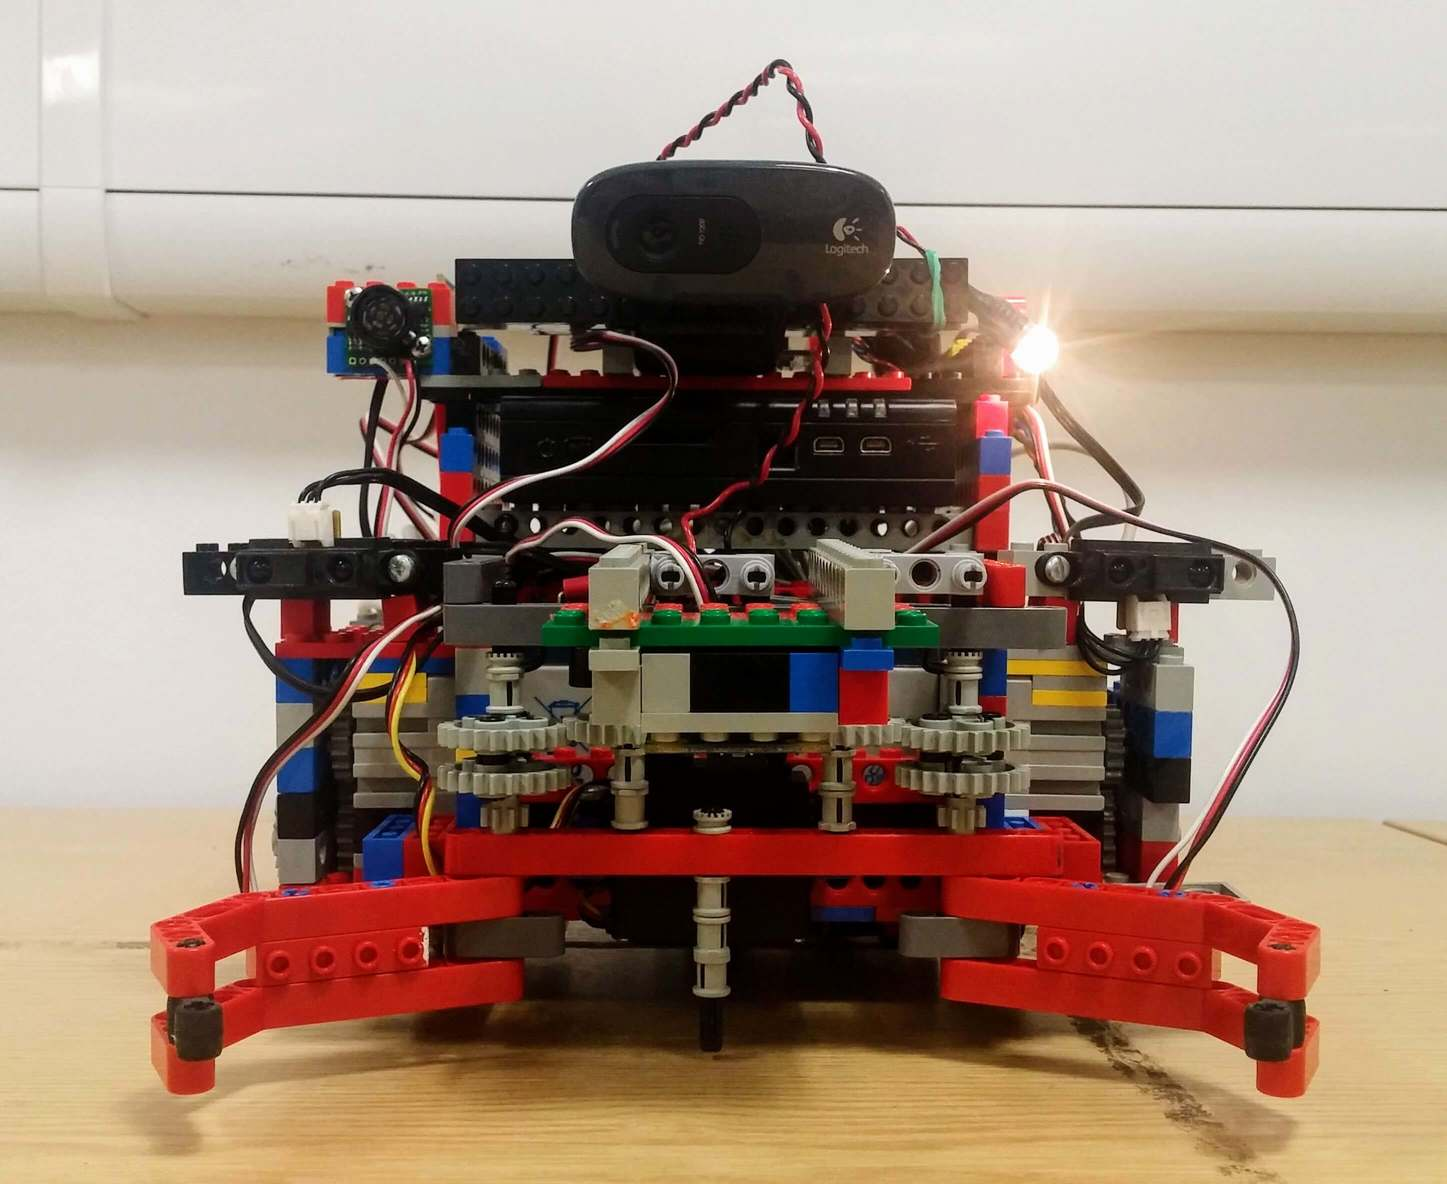
\includegraphics[width=\linewidth, height=4.5cm]{res/robot-pics/view-front.jpg}
        \caption{}
        \label{fig:}
    \end{subfigure}
    \begin{subfigure}{0.45\textwidth}
        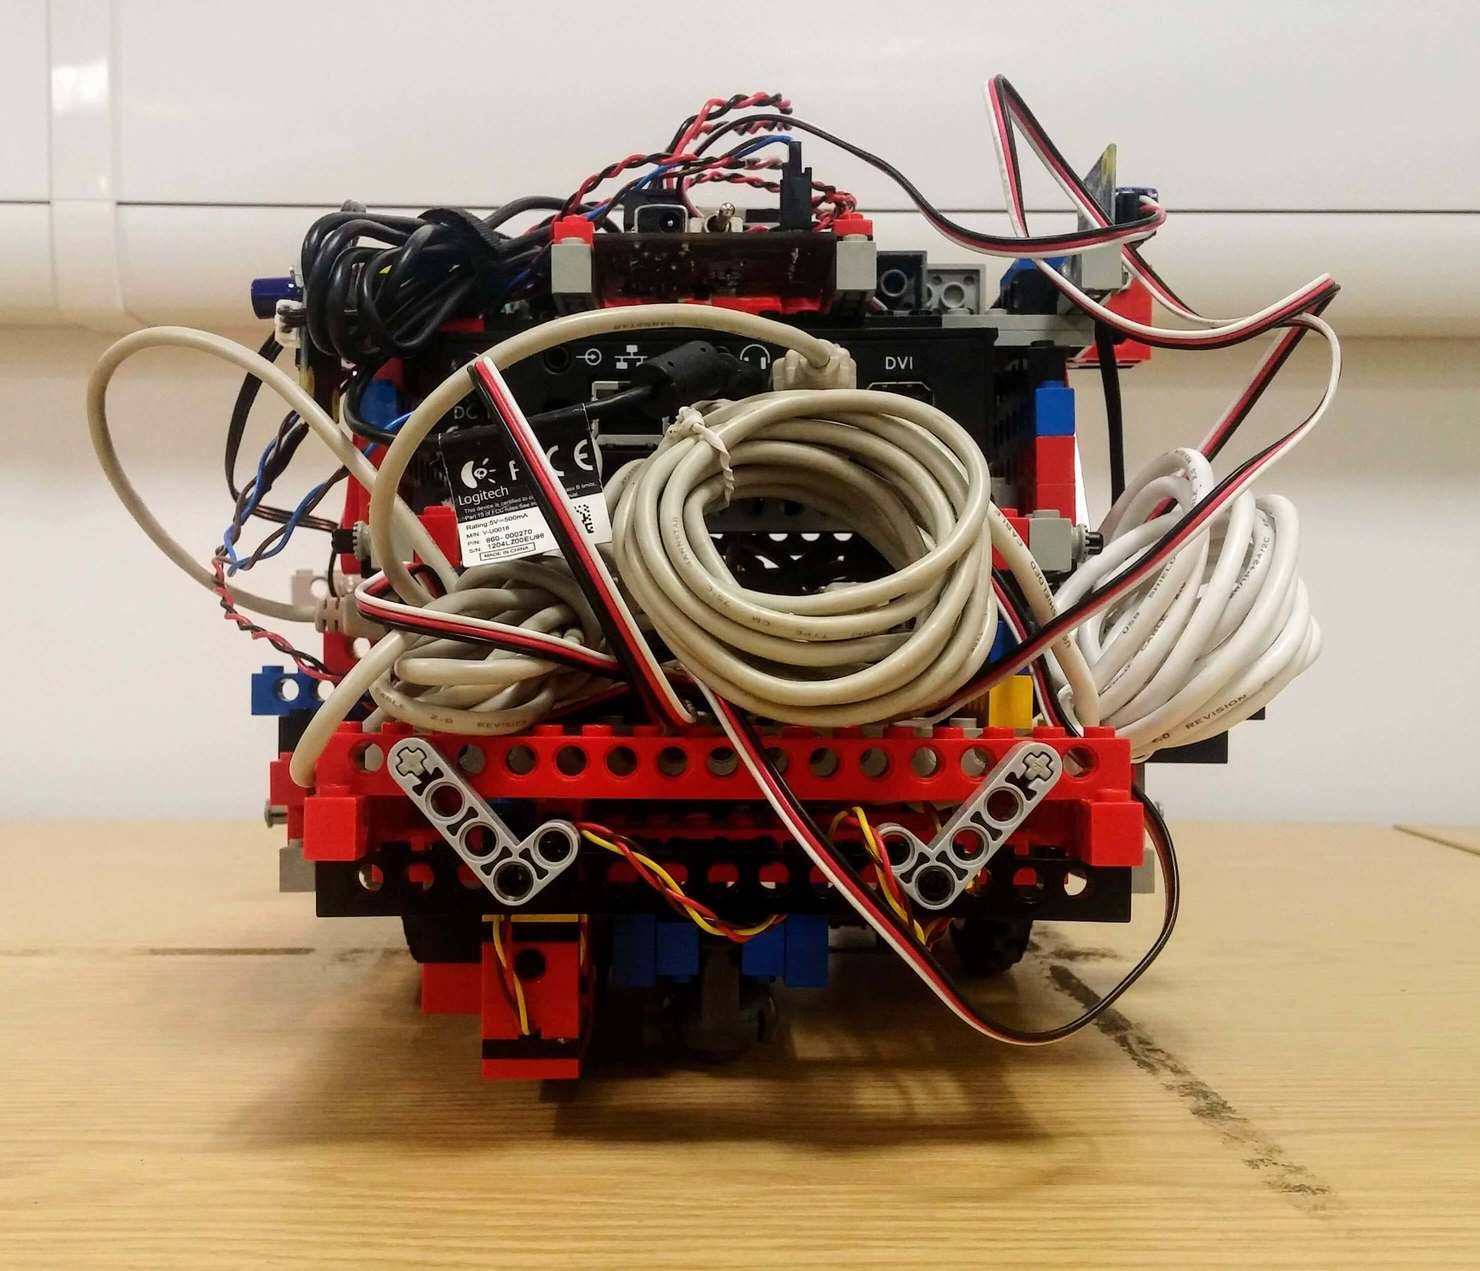
\includegraphics[width=\linewidth, height=4.5cm]{res/robot-pics/view-back.jpg}
        \caption{}
        \label{fig:}
    \end{subfigure}
    \caption{}
    \label{fig:}
\end{figure}

\begin{figure}[ht]
    \centering
    \begin{subfigure}{0.45\textwidth}
        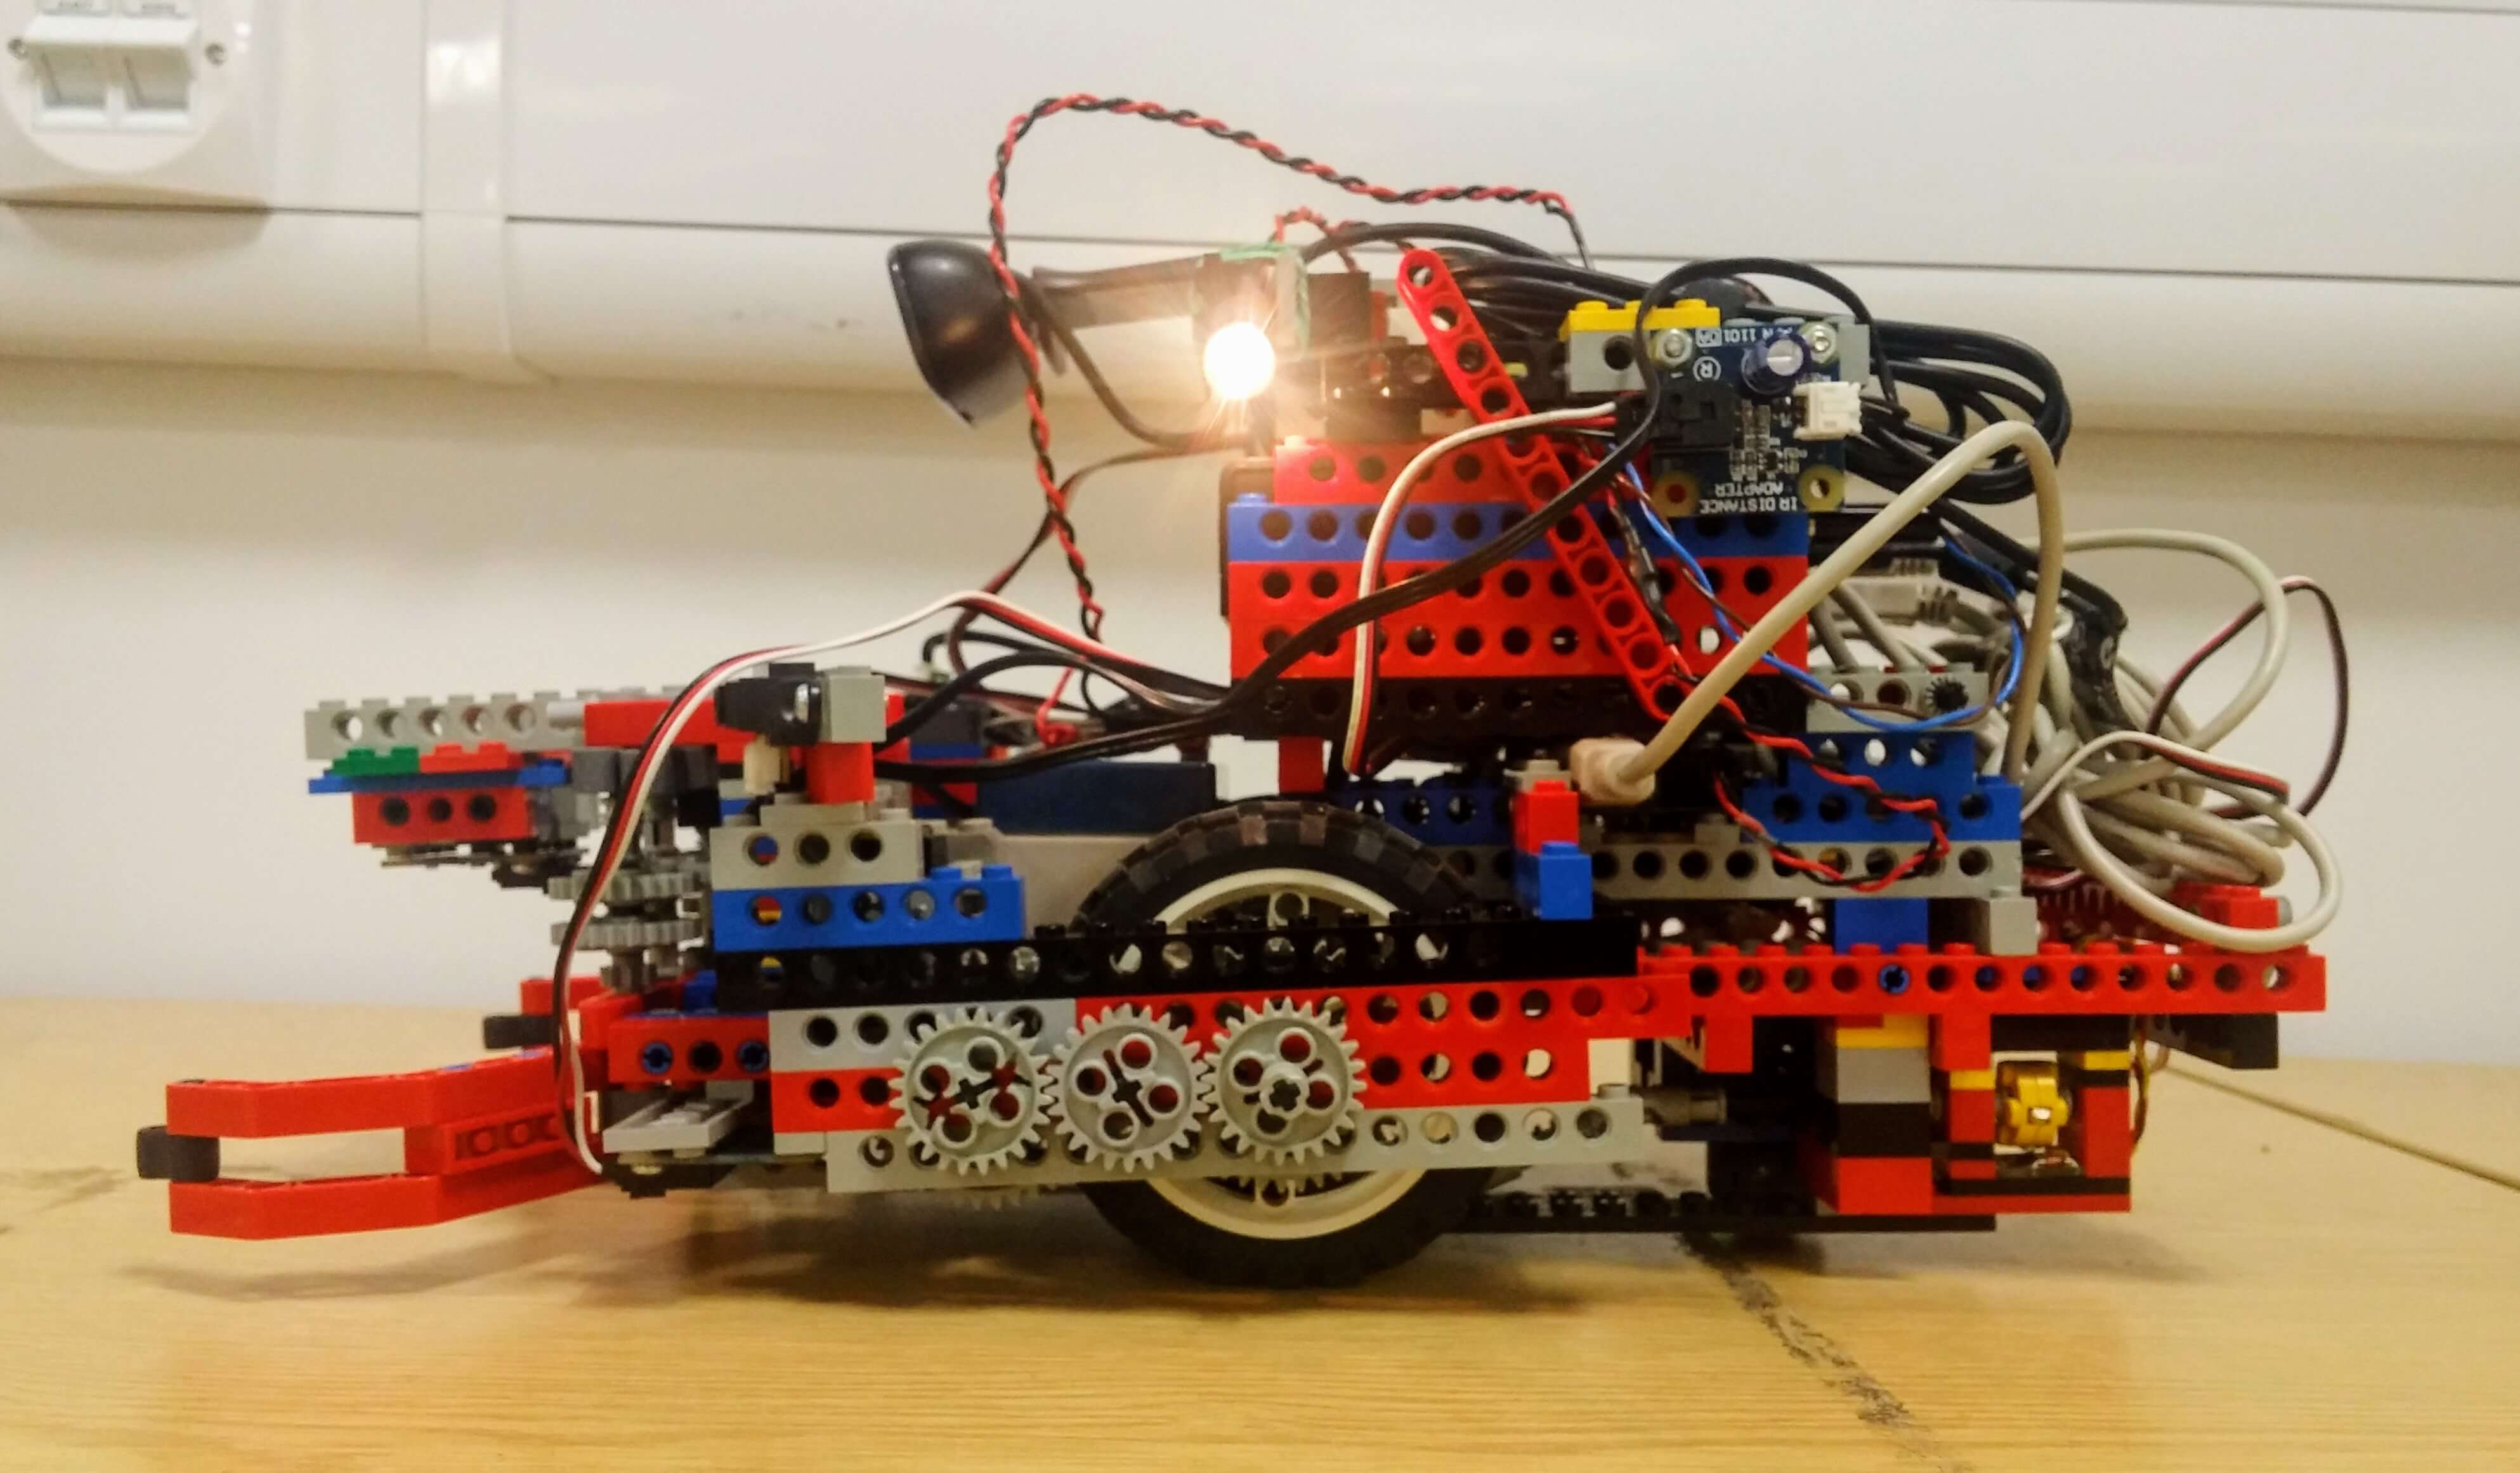
\includegraphics[width=\linewidth, height=3cm]{res/robot-pics/view-left-side.jpg}
        \caption{}
        \label{fig:}
    \end{subfigure}
    \begin{subfigure}{0.45\textwidth}
        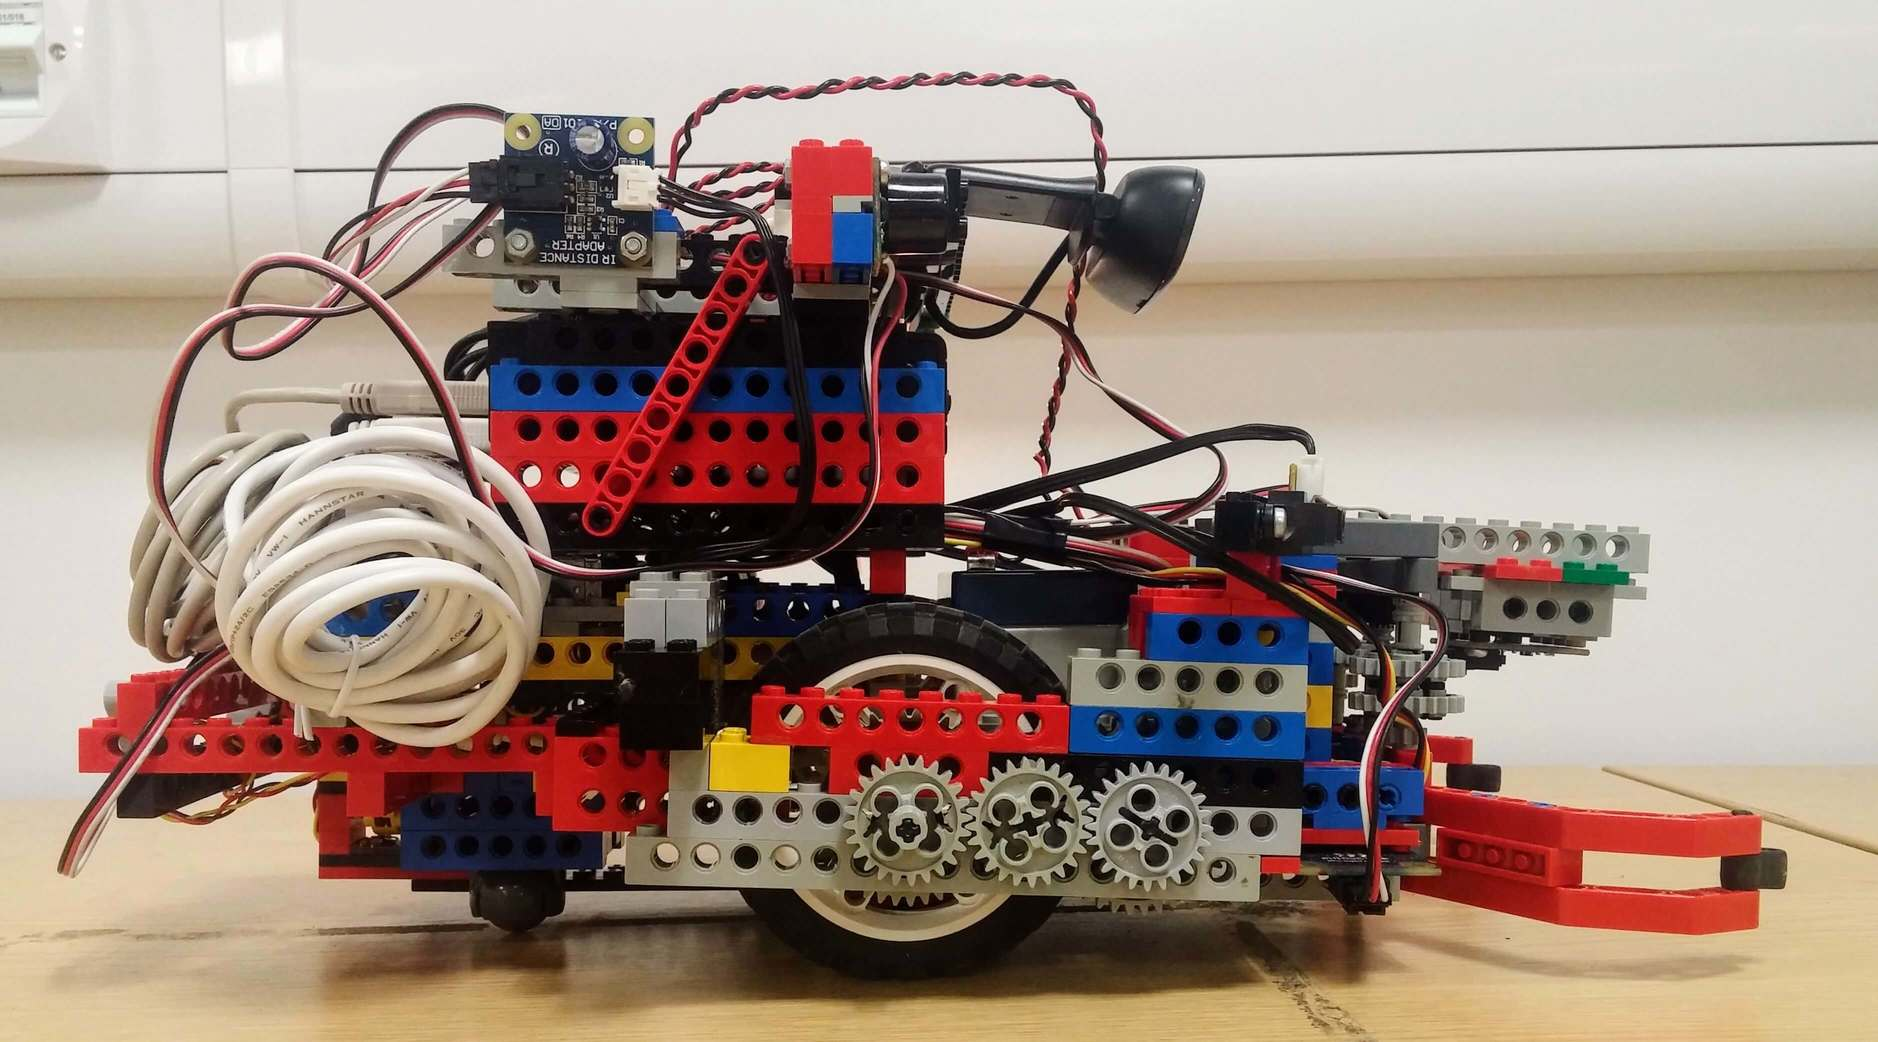
\includegraphics[width=\linewidth, height=3cm]{res/robot-pics/view-right-side.jpg}
        \caption{}
        \label{fig:}
    \end{subfigure}
    \caption{}
    \label{fig:}
\end{figure}

\begin{figure}[ht]
    \centering
    \begin{subfigure}{0.45\textwidth}
        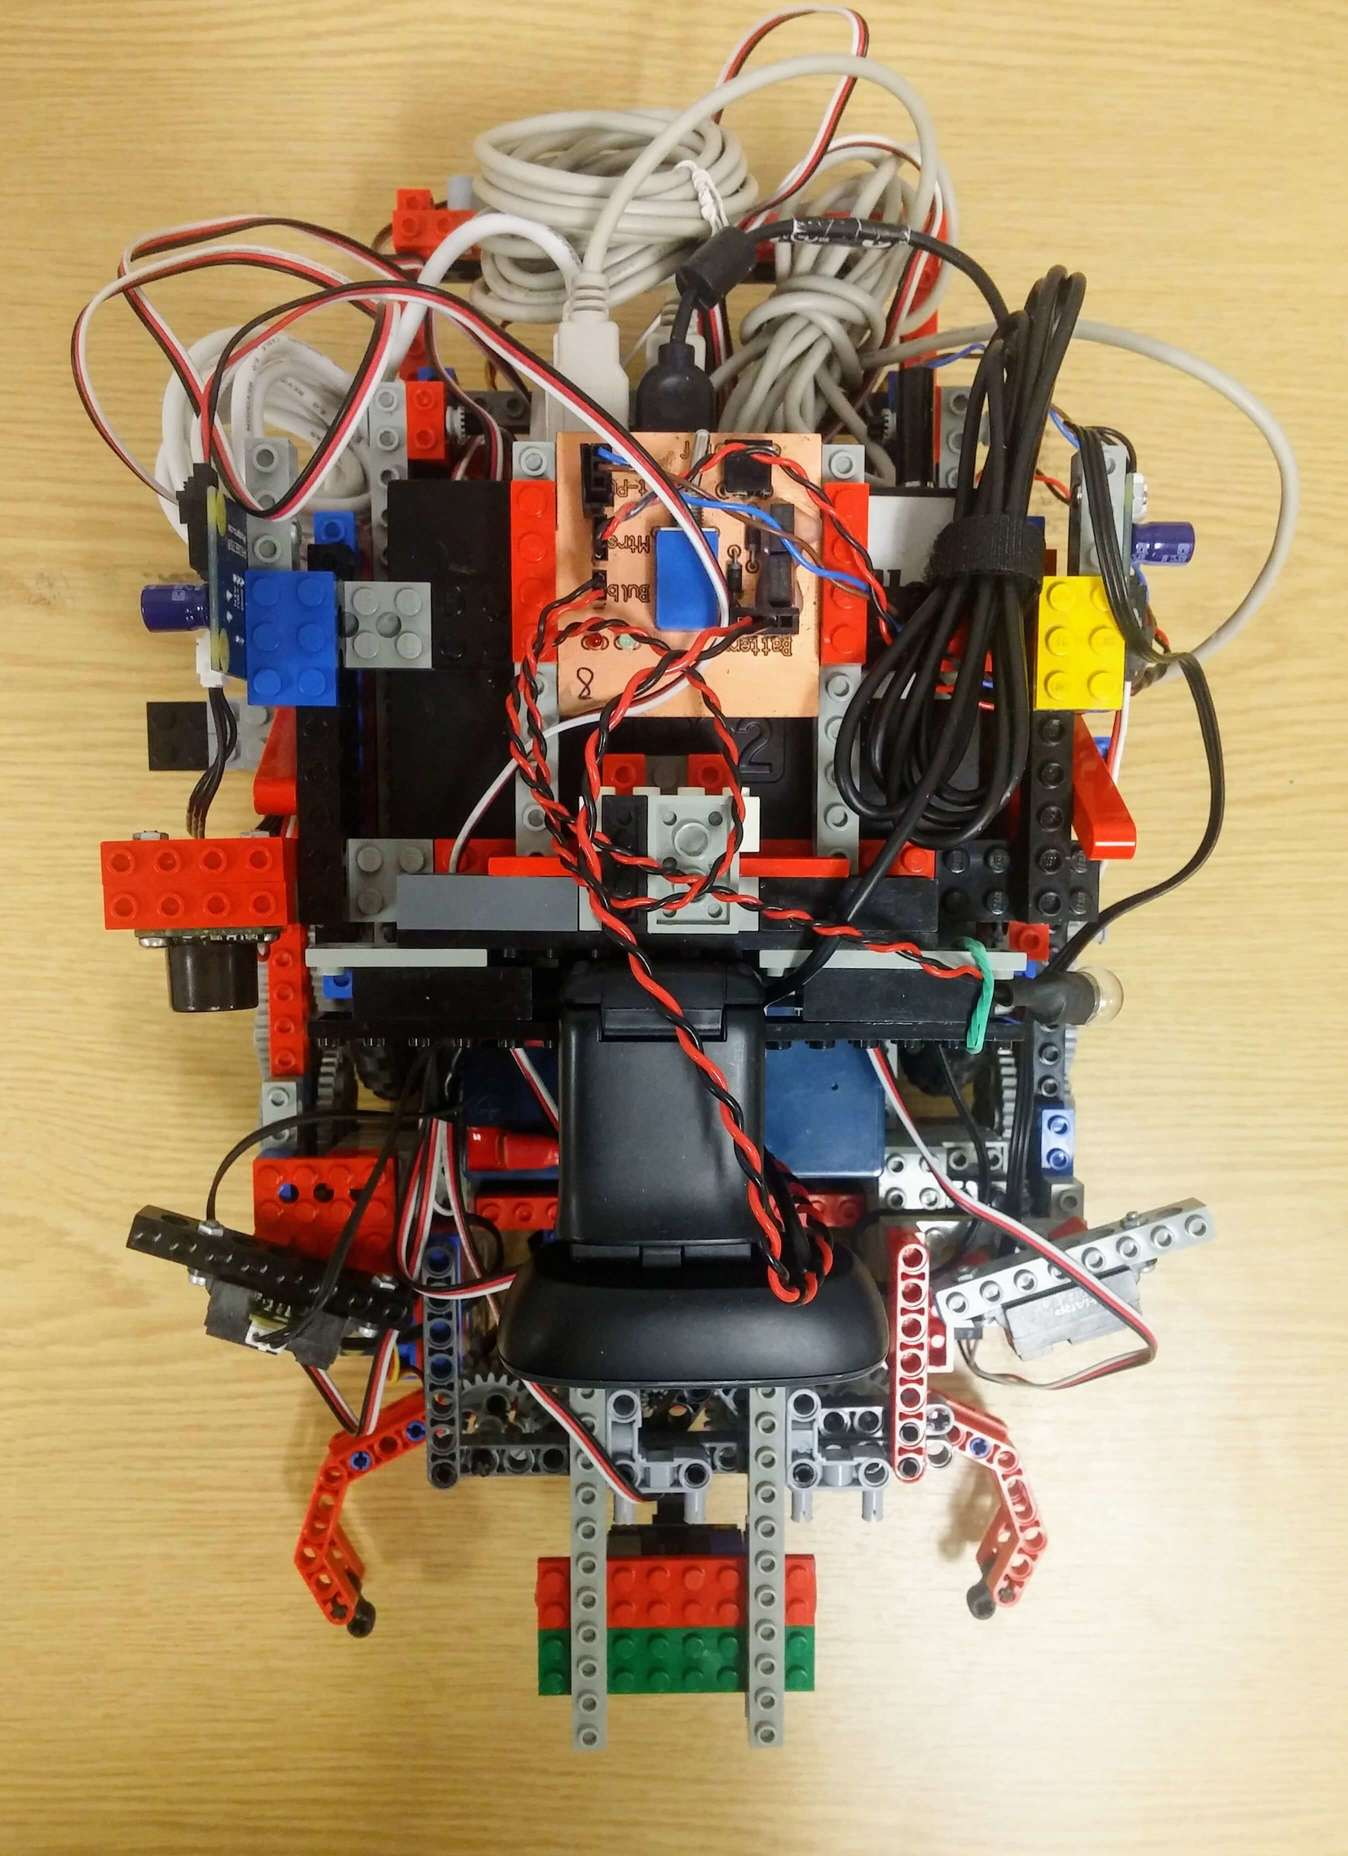
\includegraphics[width=\linewidth, height=7cm]{res/robot-pics/view-top.jpg}
        \caption{}
        \label{fig:}
    \end{subfigure}
    \begin{subfigure}{0.45\textwidth}
        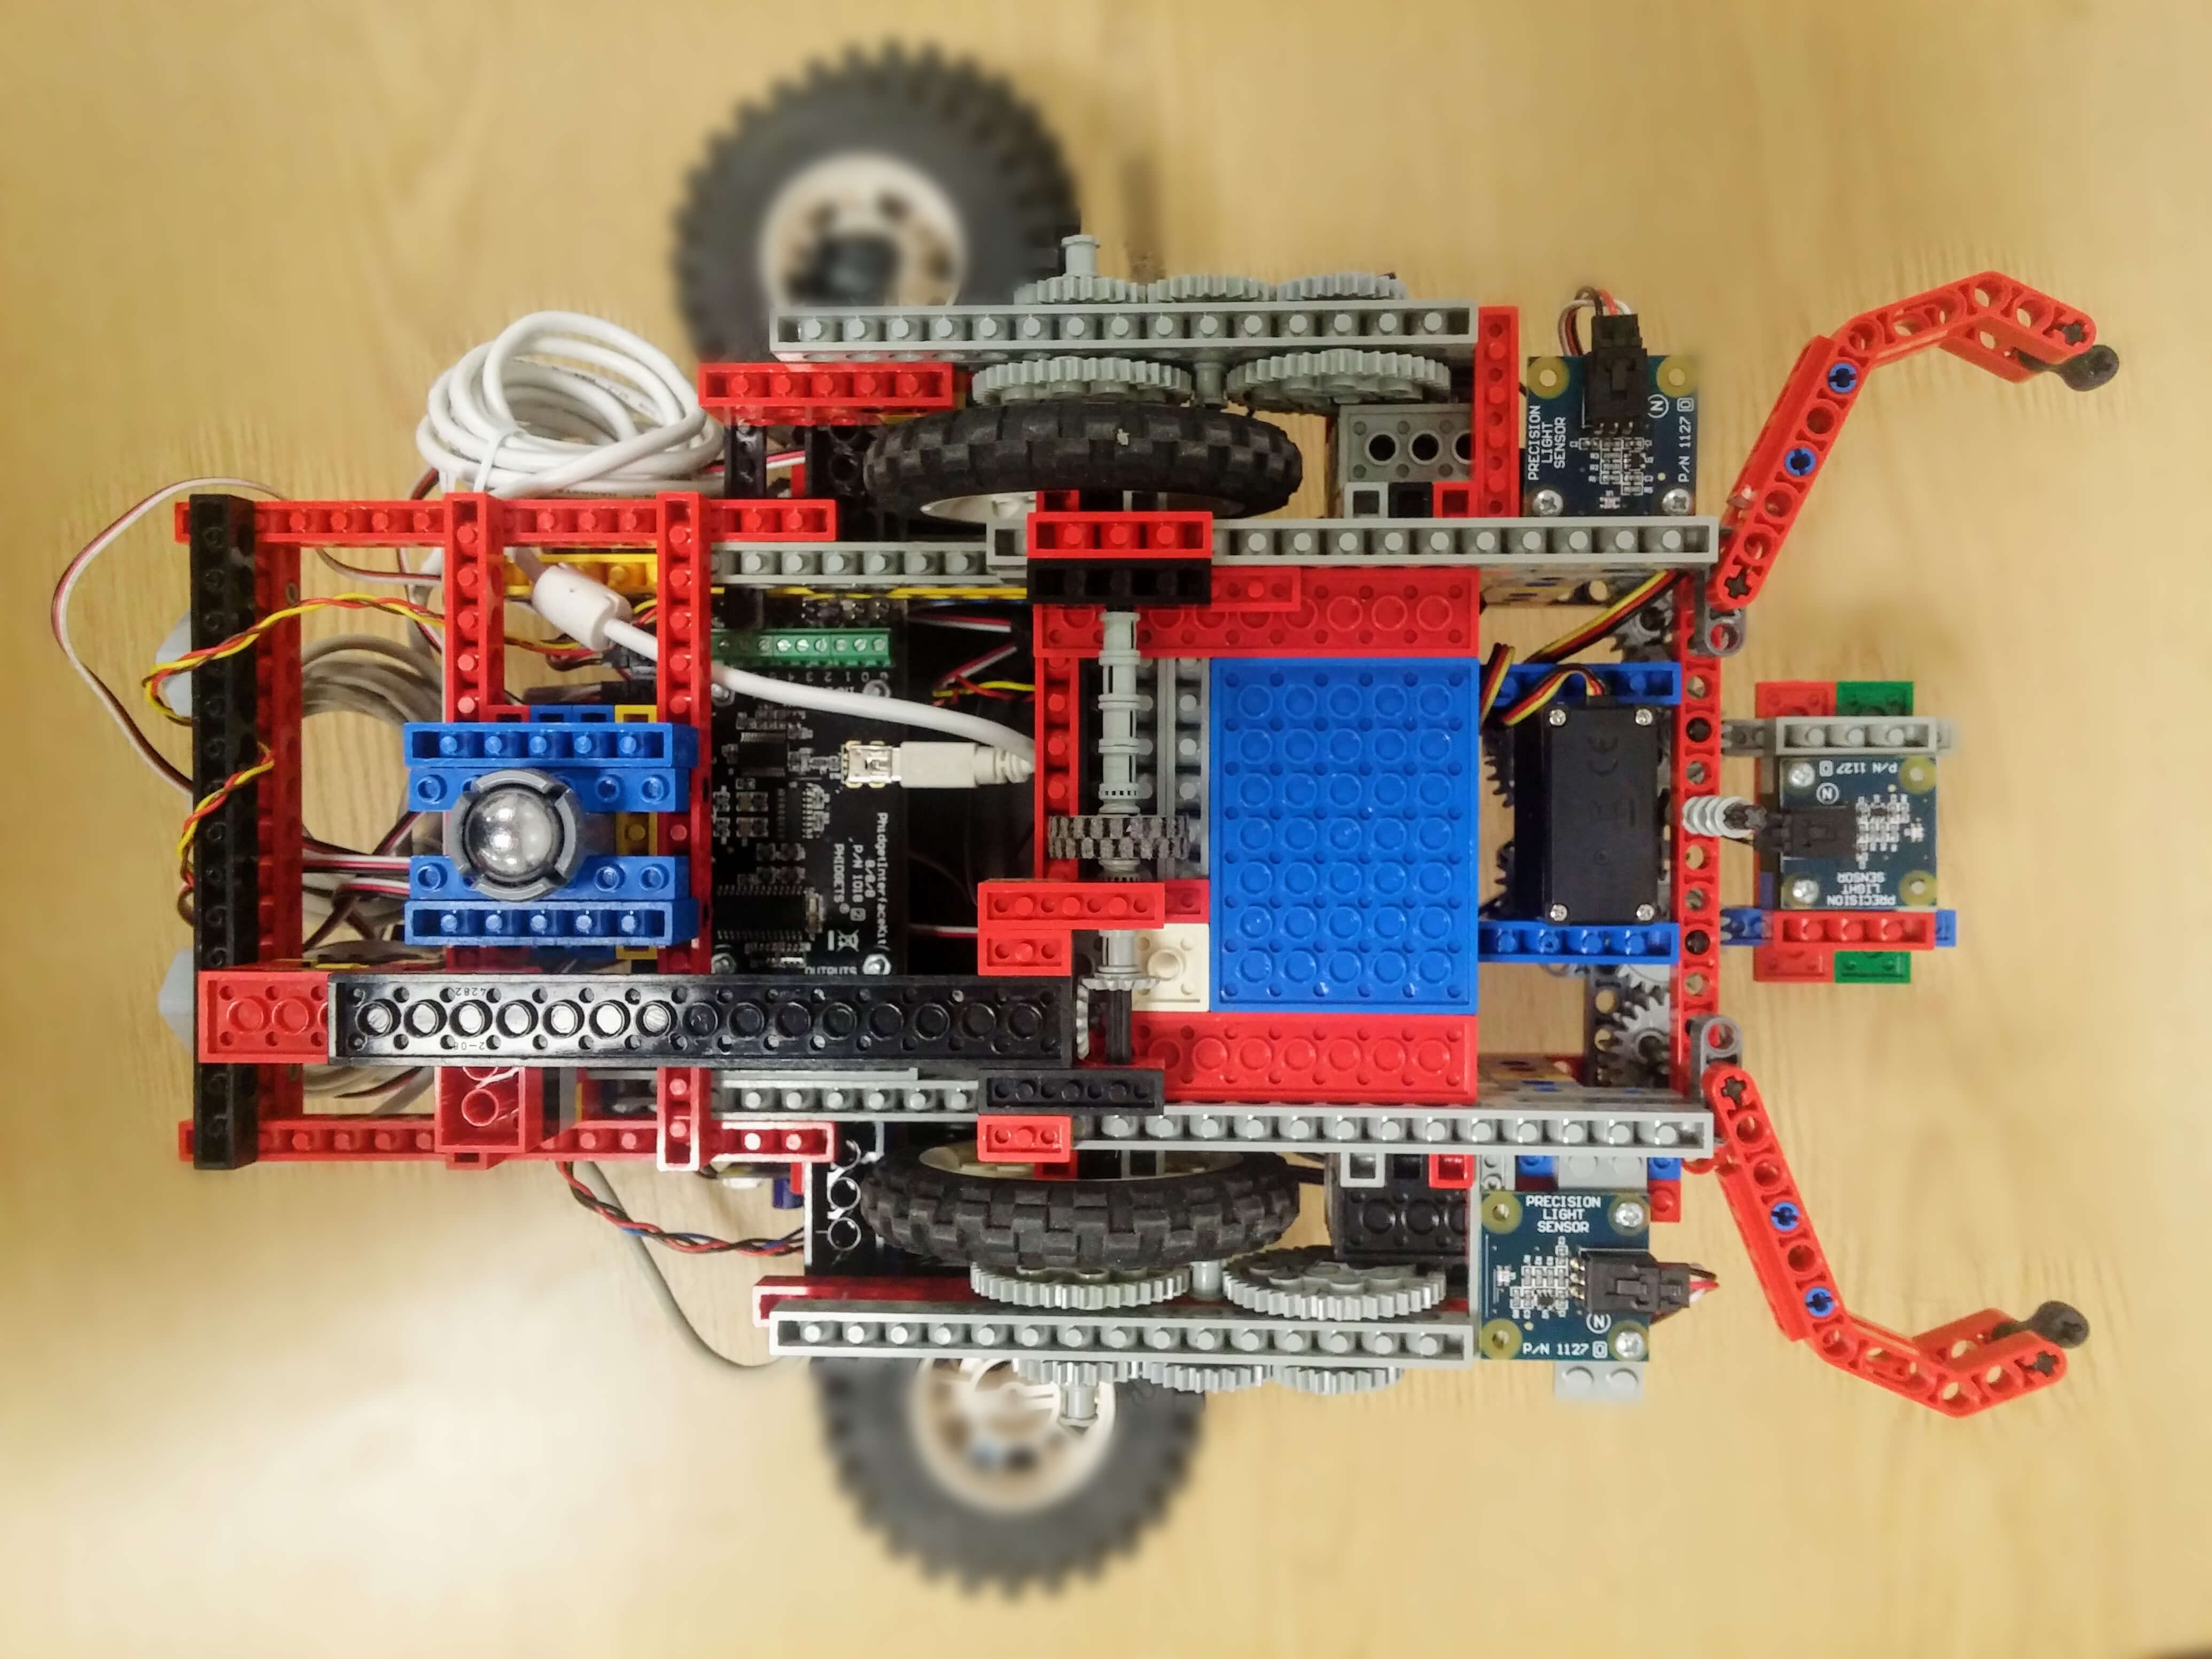
\includegraphics[width=\linewidth, height=7cm]{res/robot-pics/view-bottom.jpg}
        \caption{}
        \label{fig:}
    \end{subfigure}
    \caption{}
    \label{fig:}
\end{figure}

\begin{figure}[ht]
    \centering
    \begin{subfigure}{0.45\textwidth}
        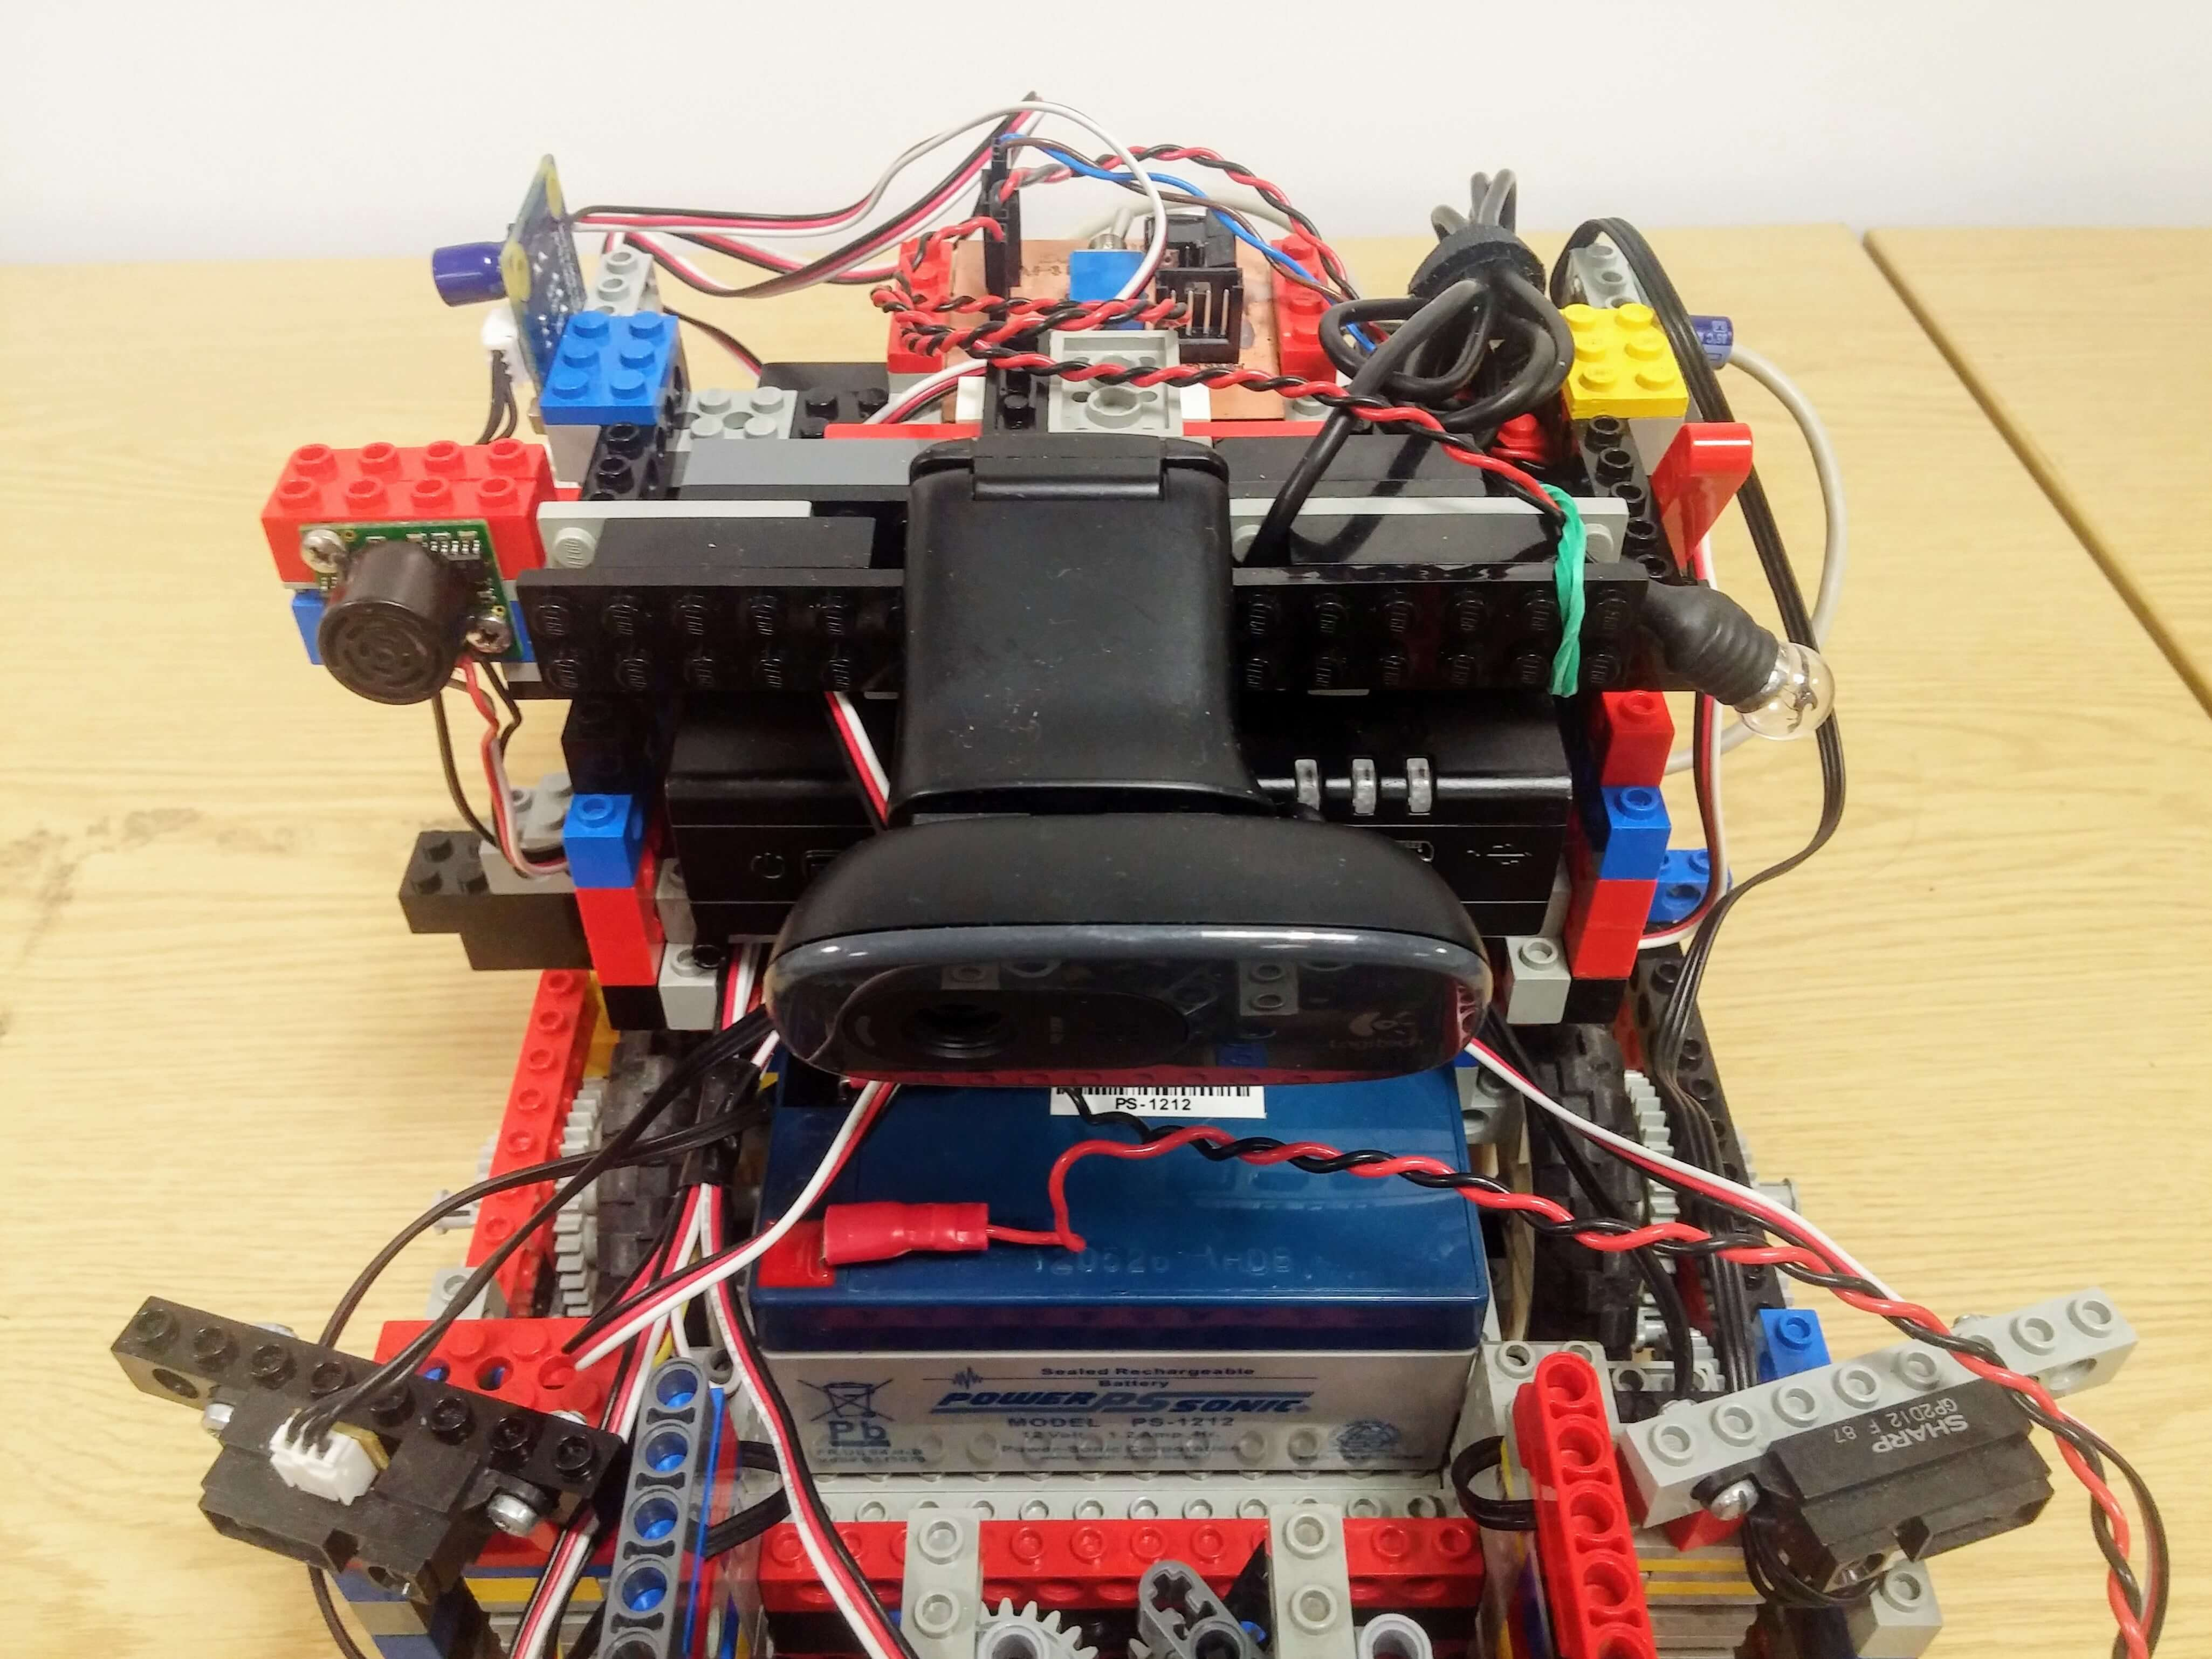
\includegraphics[width=\linewidth, height=4cm]{res/robot-pics/top-on.jpg} 
        \caption{Hop on}
        \label{fig:hop-on}
    \end{subfigure}
    \begin{subfigure}{0.45\textwidth}
        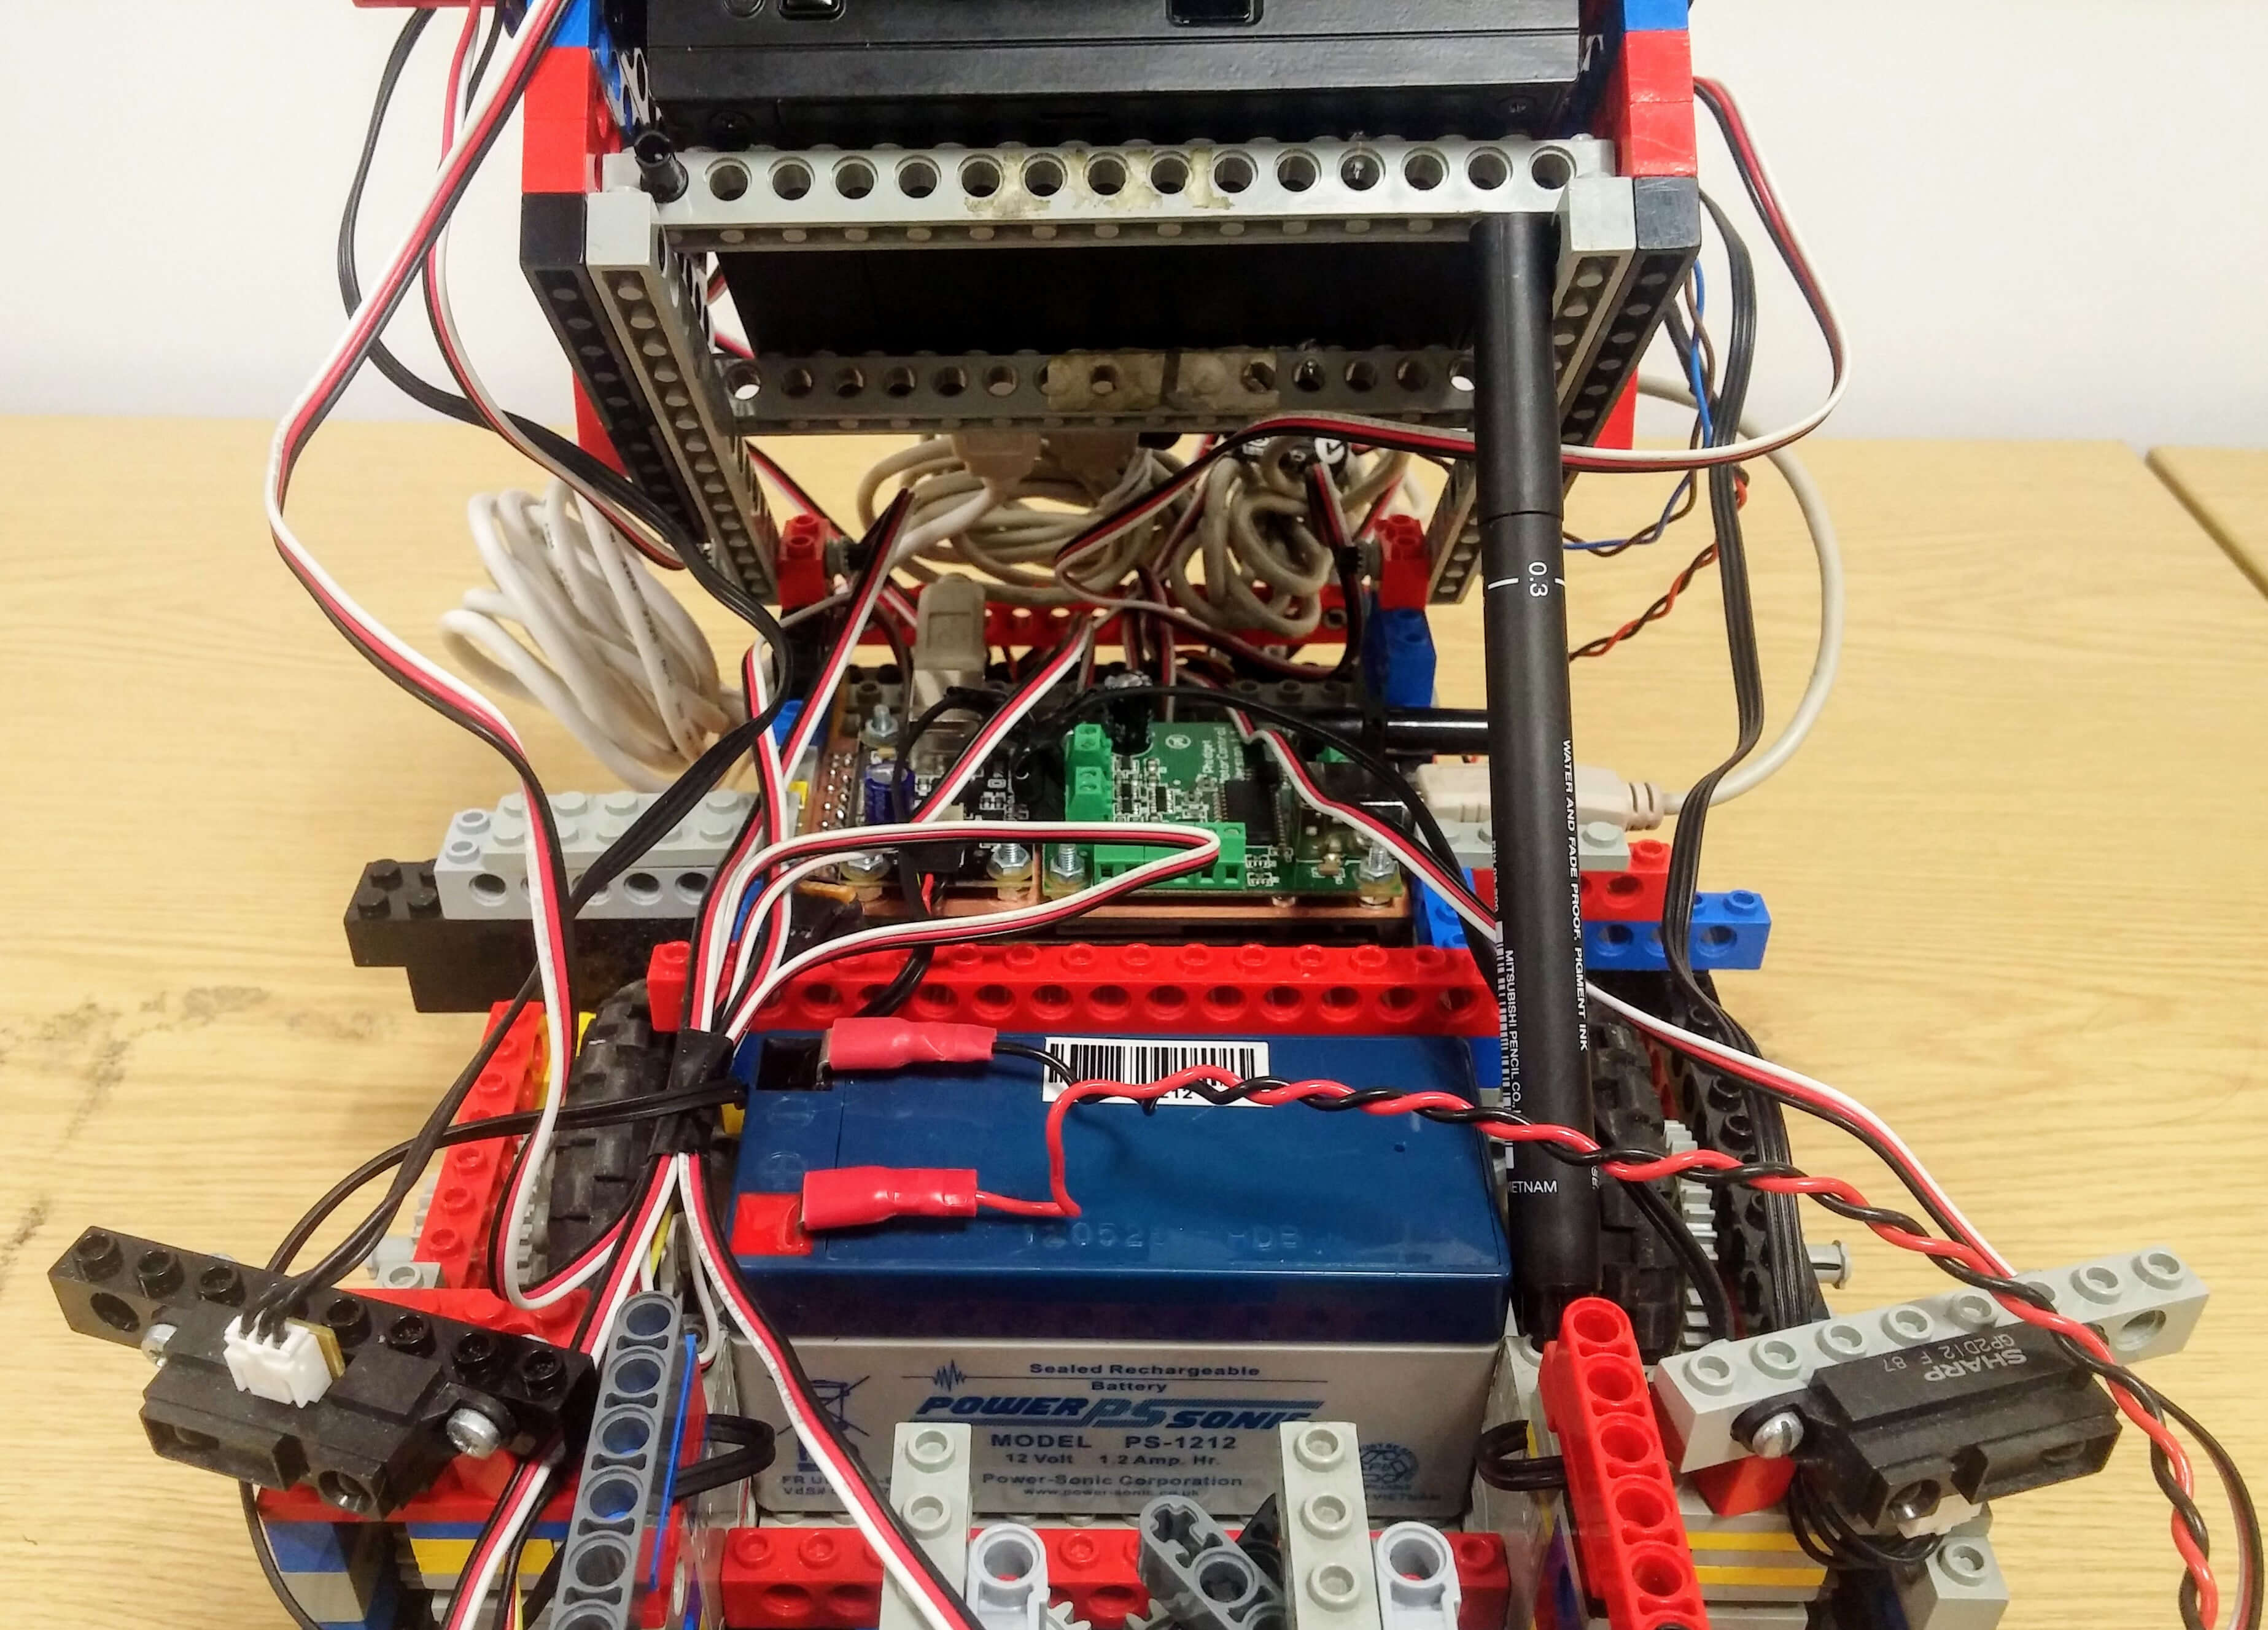
\includegraphics[width=\linewidth, height=4cm]{res/robot-pics/top-off.jpg}
        \caption{Hop off}
        \label{fig:hop-off}
    \end{subfigure}
    \caption{Lifting the hop reveals the Phidgets boards and enables easy access to the battery slot.}
    \label{fig:hop-on-off}
\end{figure}

% - - - - - - - - - - - - - - - - - - - - - - - - - - -

\subsection{Base detector and gripper}

\begin{figure}[ht]
    \centering
    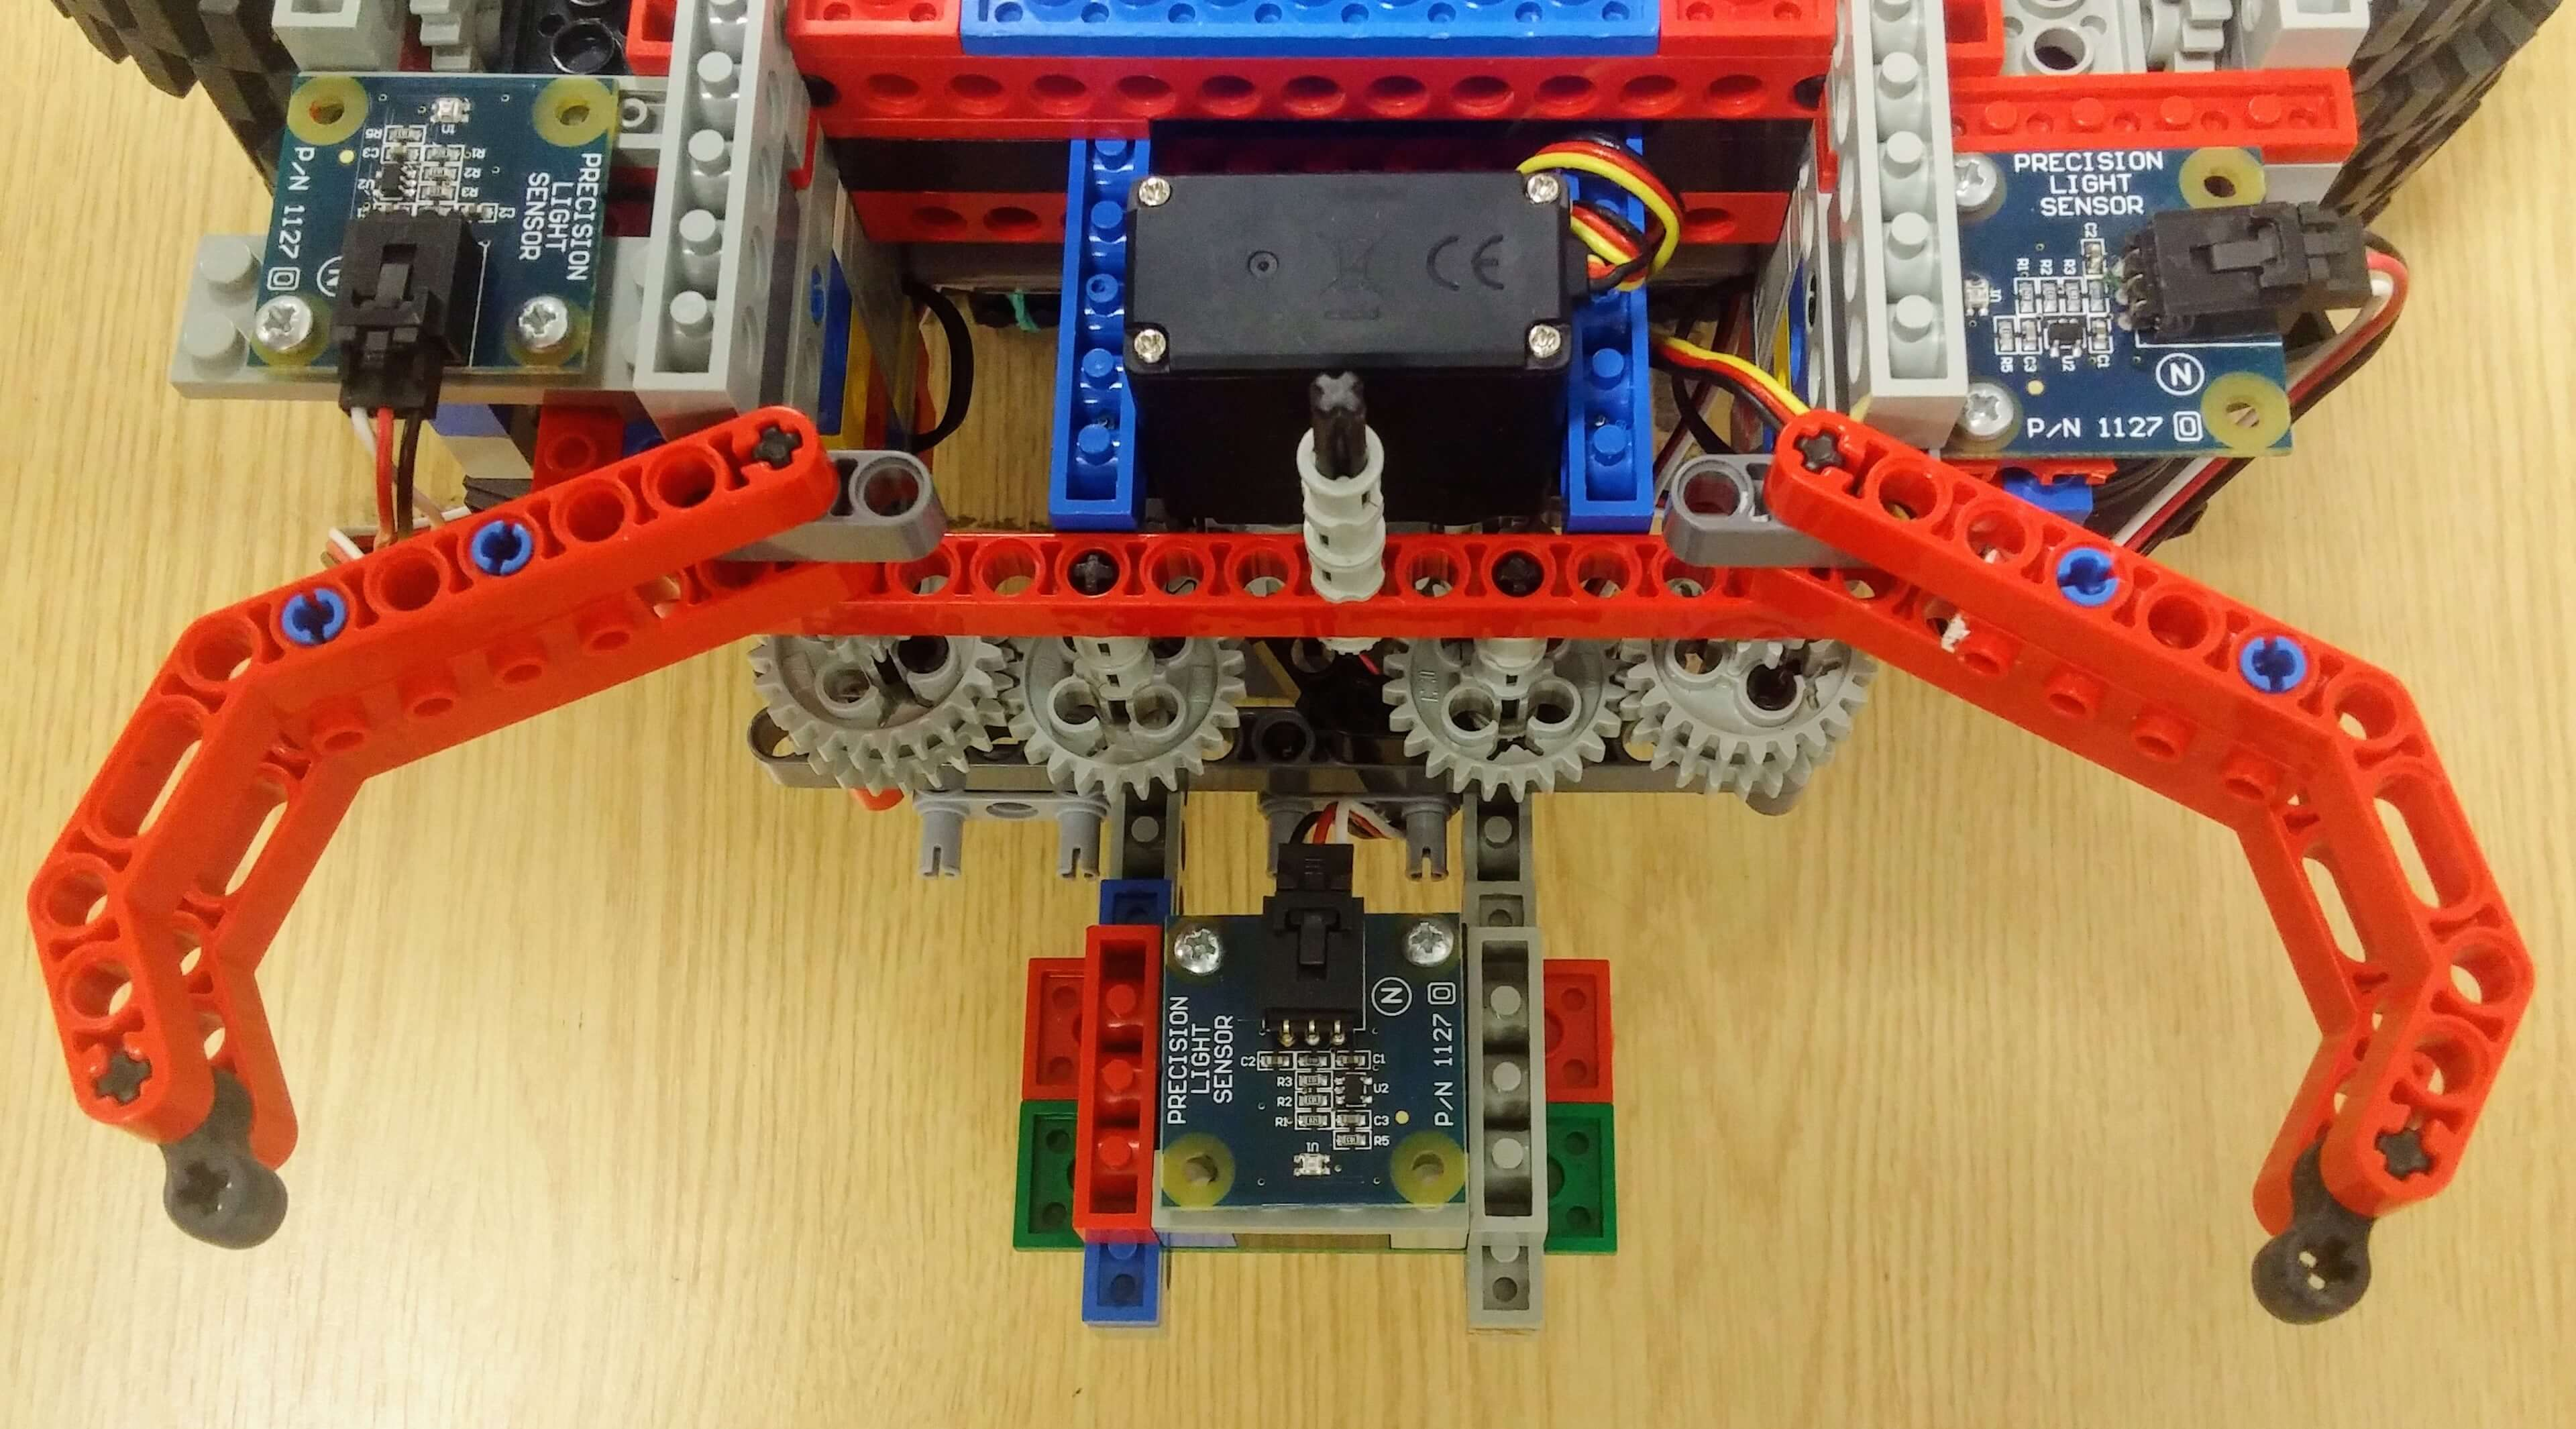
\includegraphics[width=0.7\linewidth]{res/robot-pics/base-detector-and-gripper.jpg}
    \caption{}
    \label{fig:}
\end{figure}

% - - - - - - - - - - - - - - - - - - - - - - - - - - -

\subsection{Actuators and gearing}

\begin{figure}[ht]
    \centering
    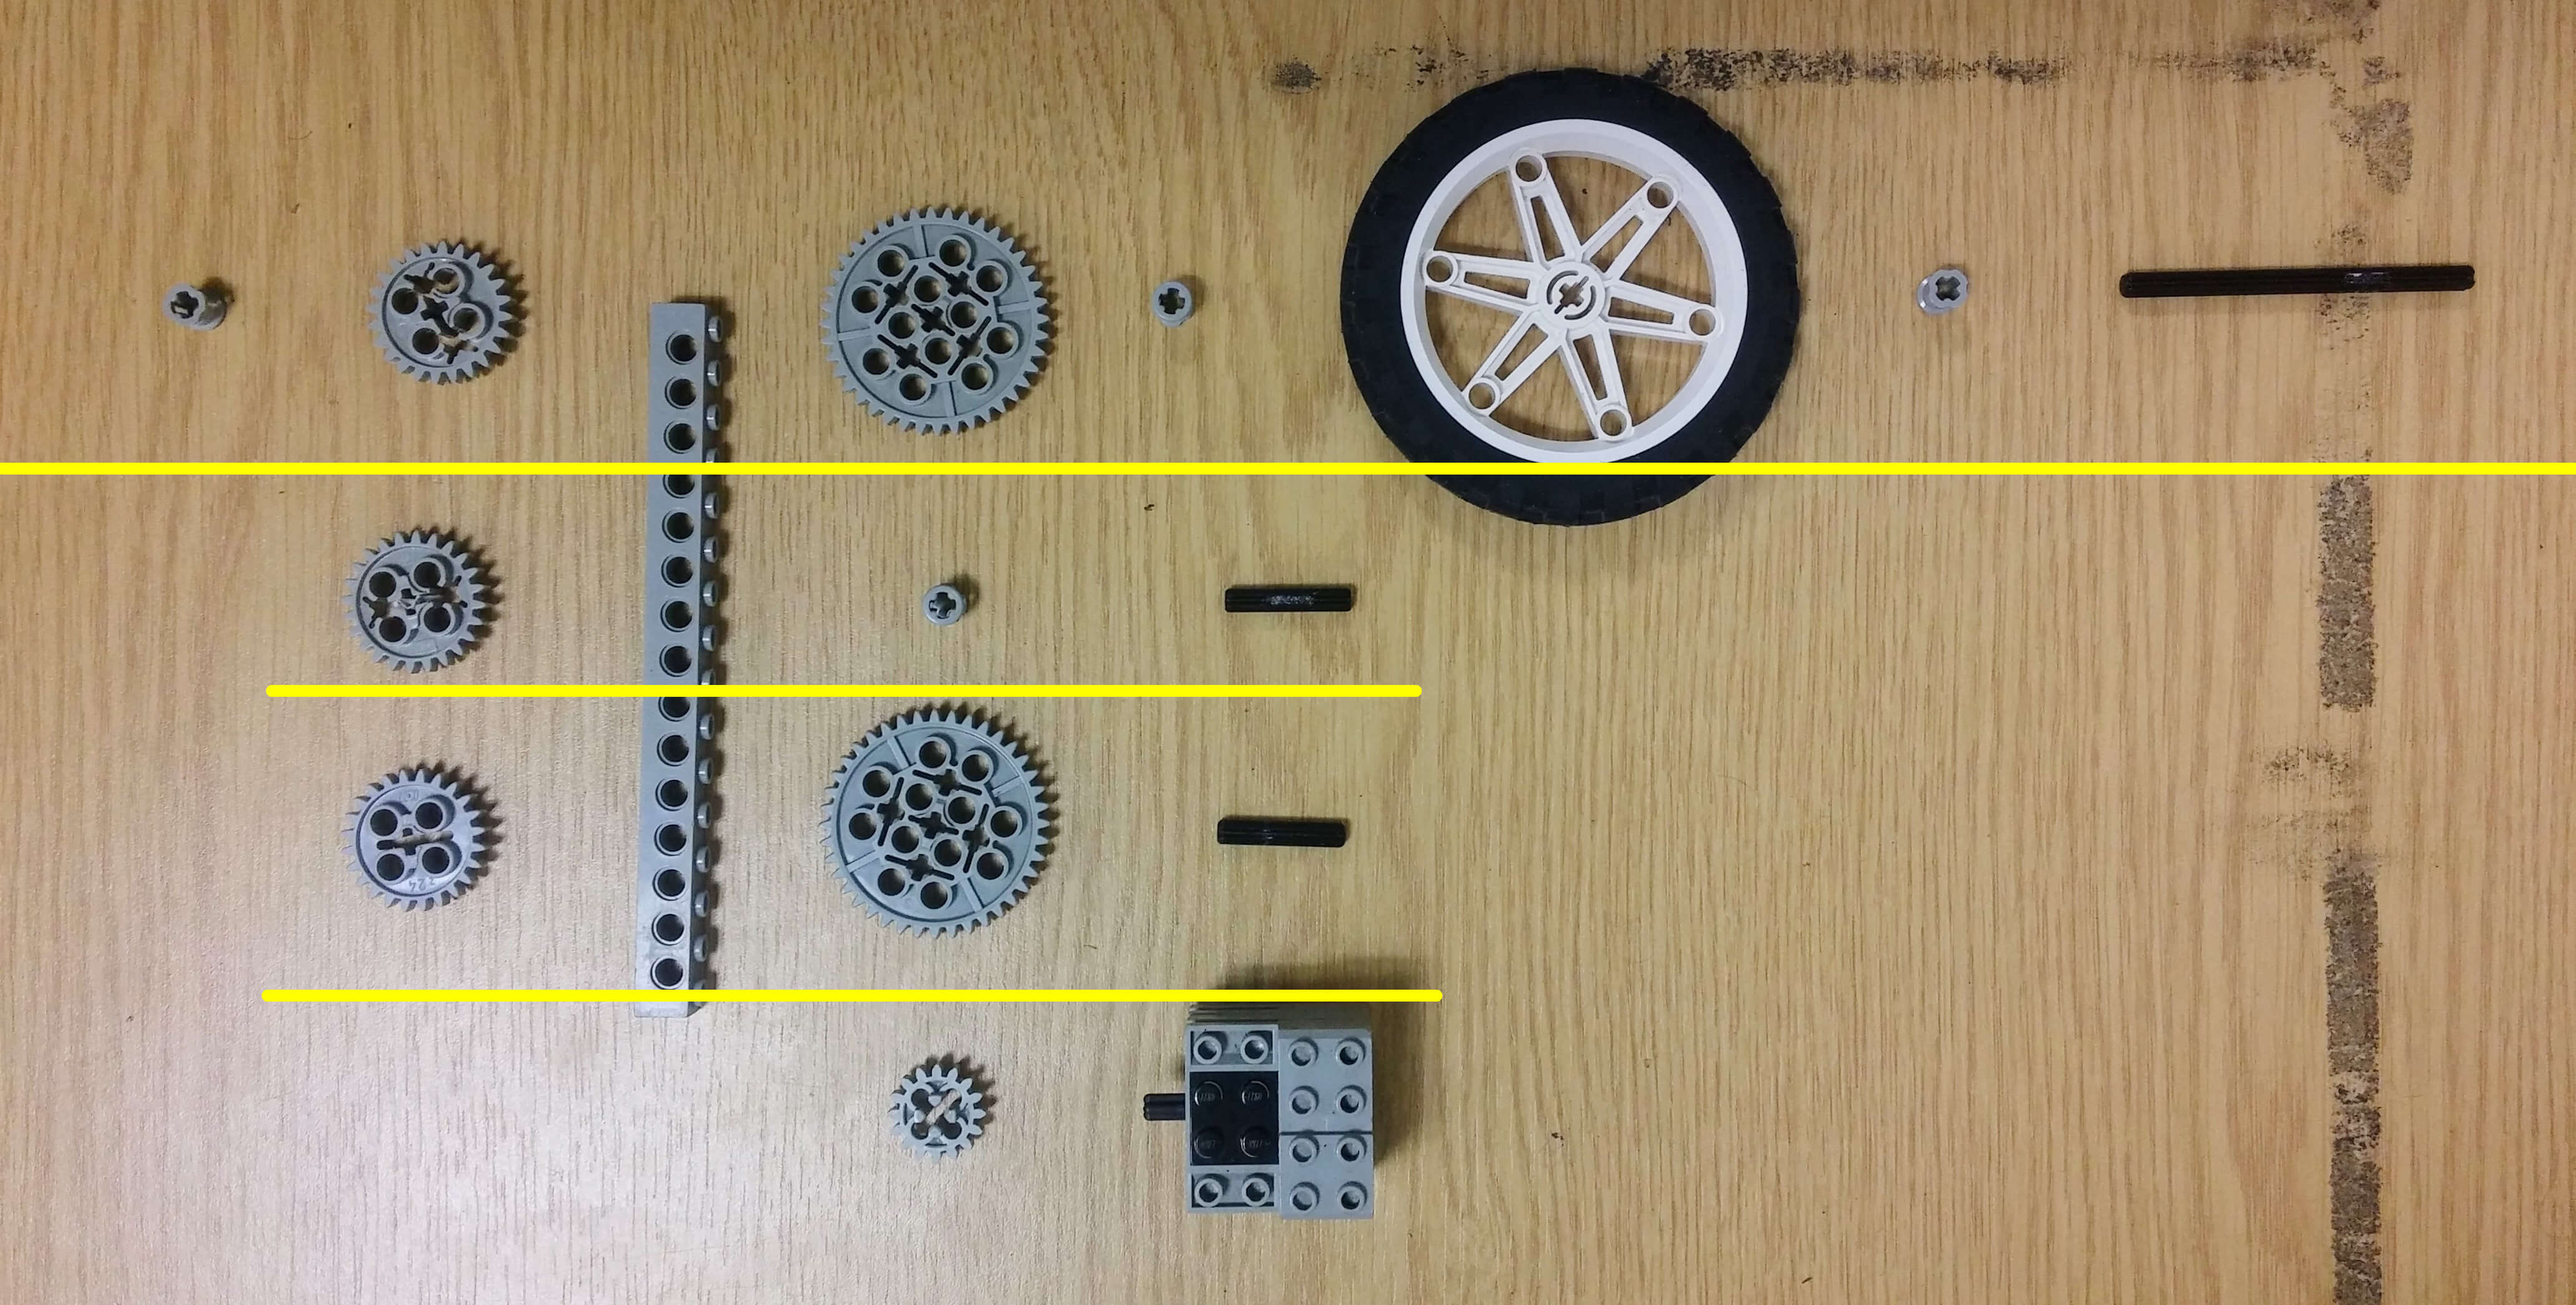
\includegraphics[width=0.7\linewidth]{res/robot-pics/gear-train-unmounted.jpg}
    \caption{}
    \label{fig:}
\end{figure}

\begin{figure}[ht]
    \centering
    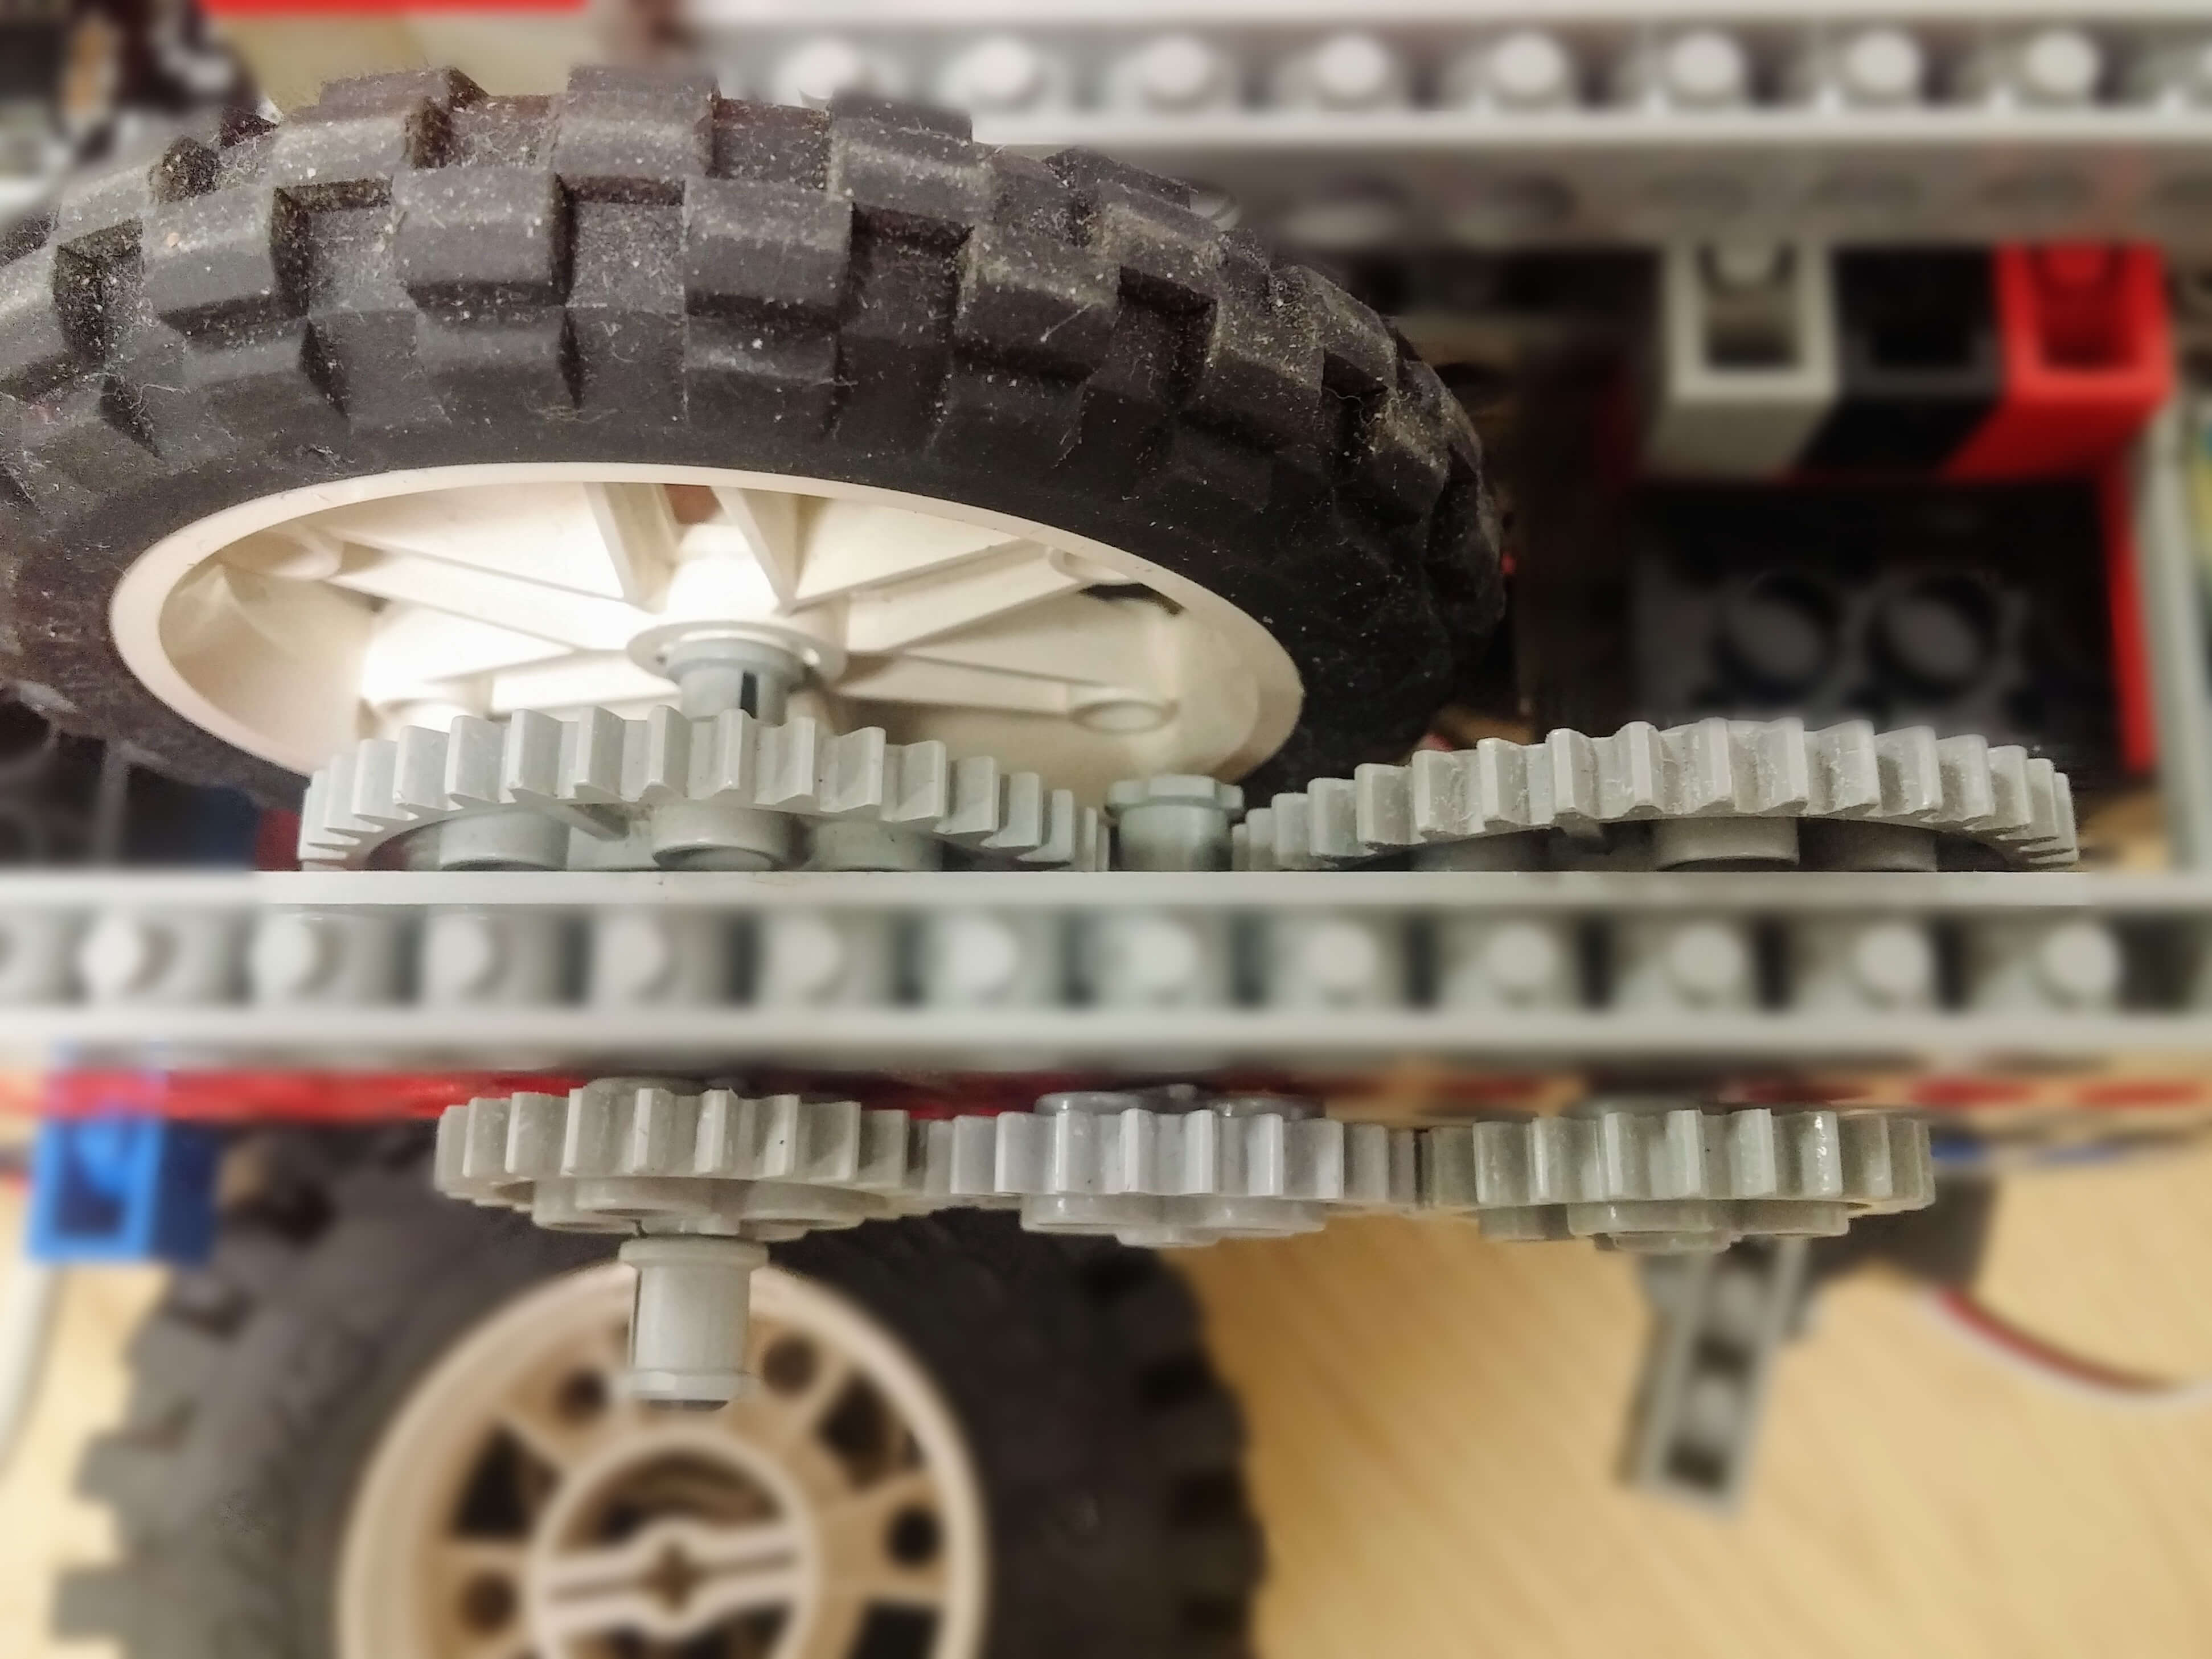
\includegraphics[width=0.7\linewidth]{res/robot-pics/gear-train-mounted.jpg}
    \caption{}
    \label{fig:}
\end{figure}

% - - - - - - - - - - - - - - - - - - - - - - - - - - -

\subsection{Sensing}

\subsubsection{IR and Sonar}

\begin{figure}[ht]
    \centering
    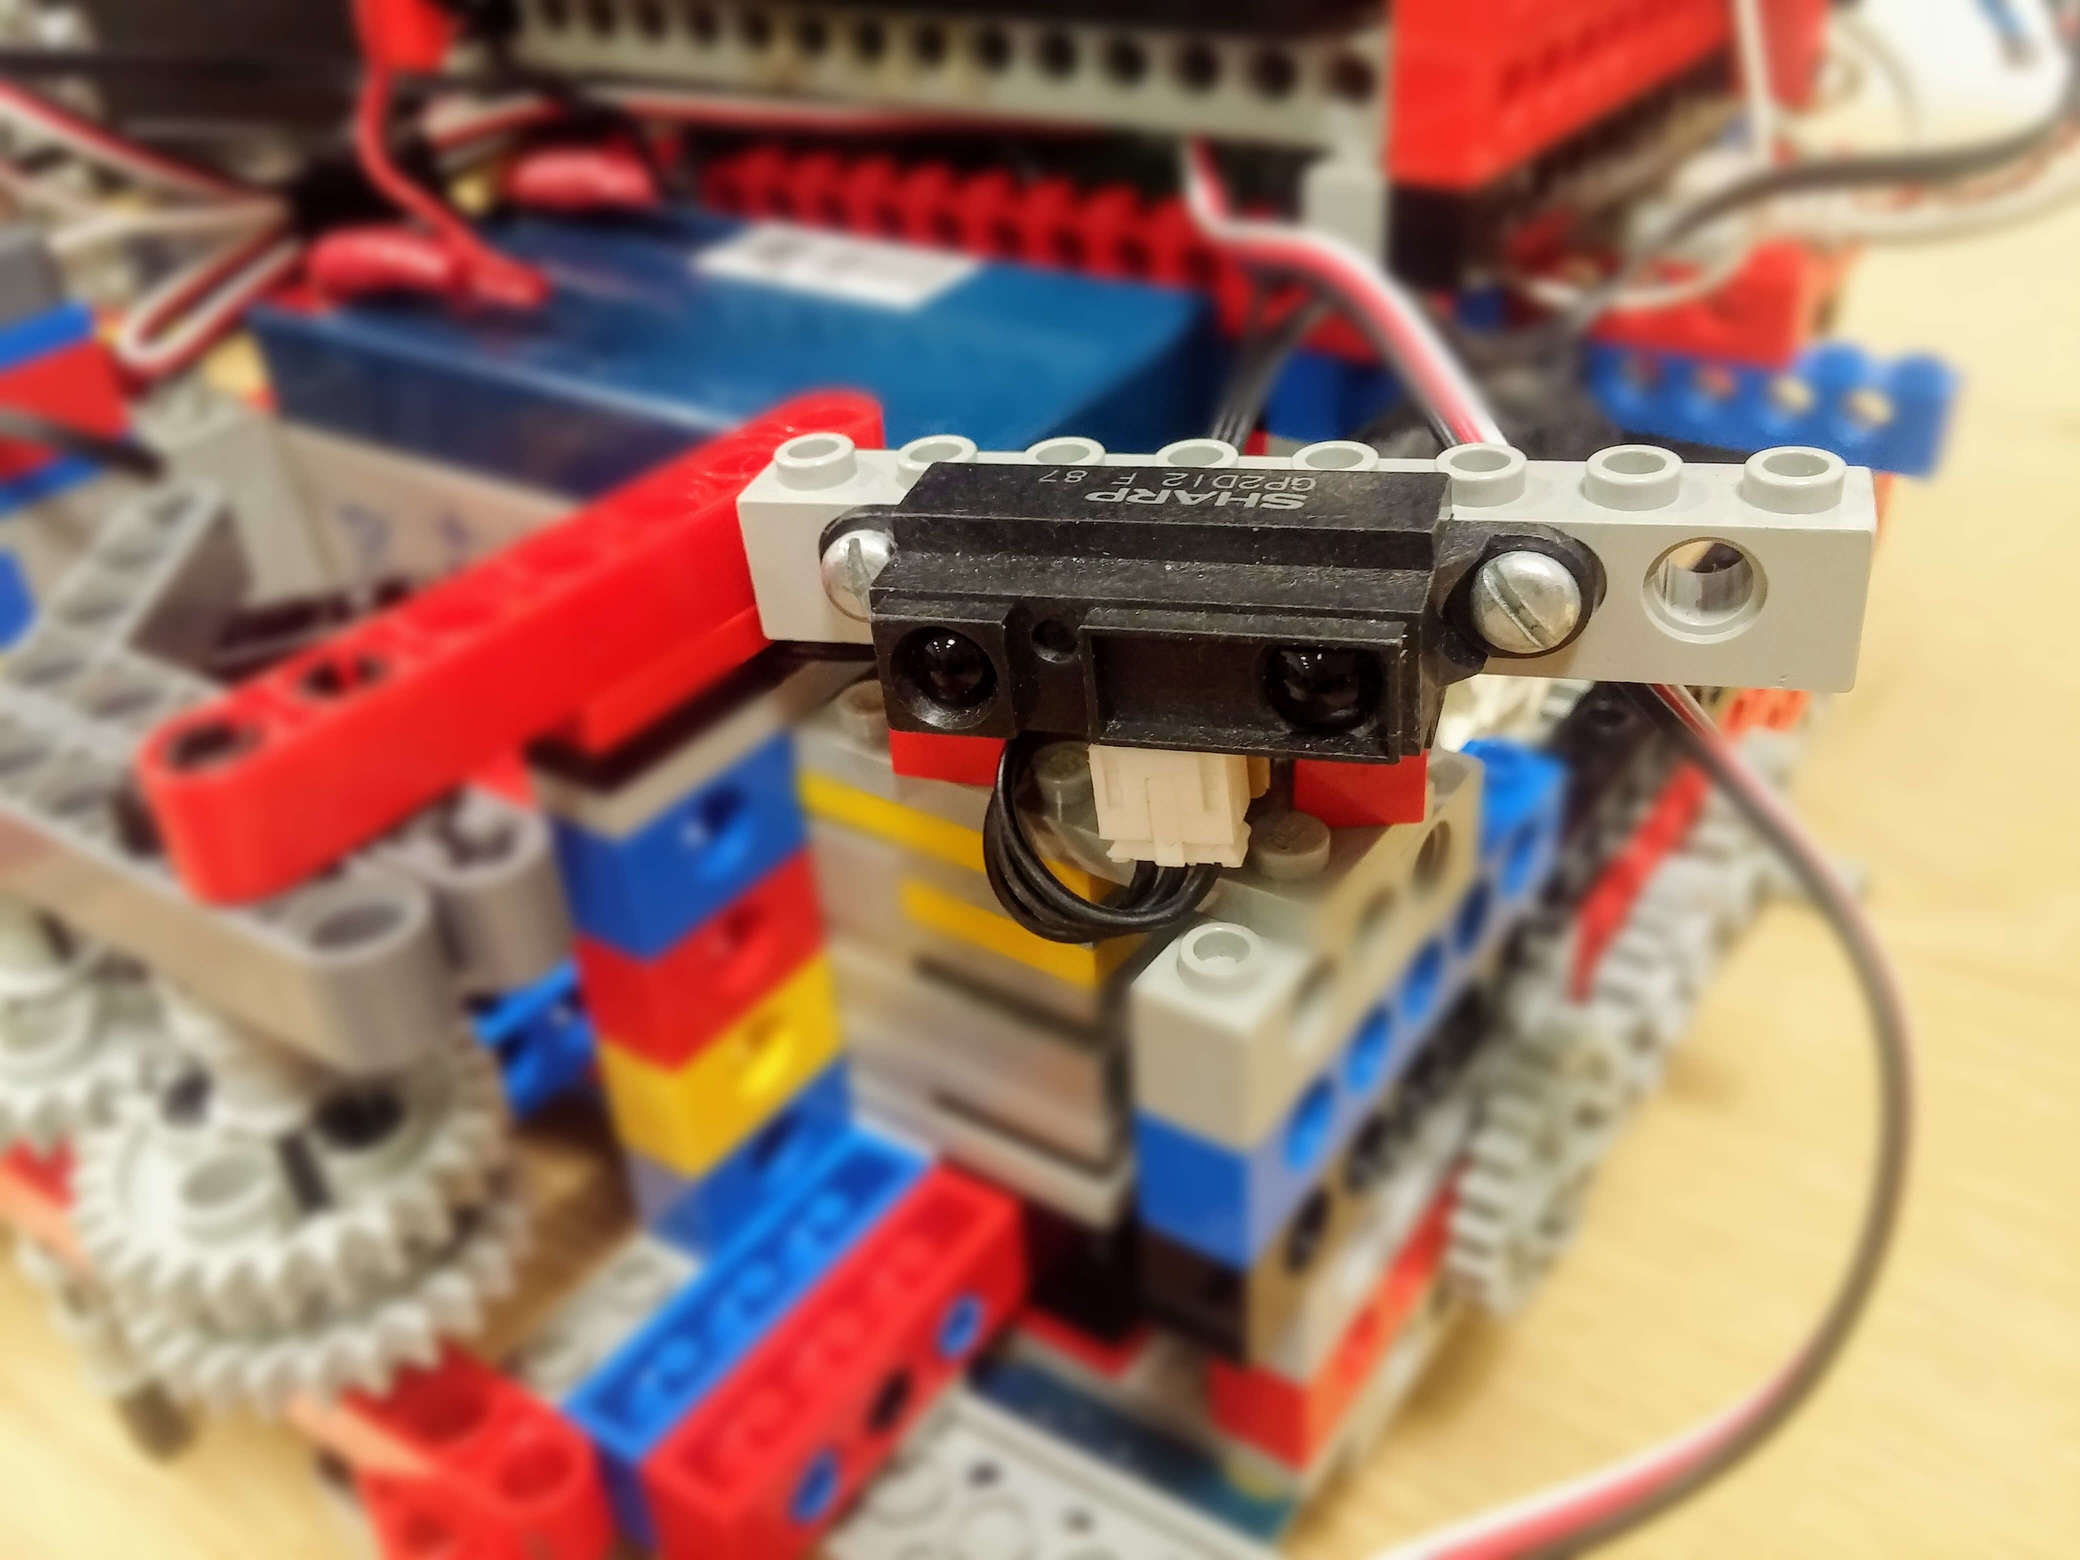
\includegraphics[width=0.7\linewidth]{res/robot-pics/ir-sensor-placement.jpg}
    \caption{}
    \label{fig:}
\end{figure}

\begin{figure}[ht]
    \centering
    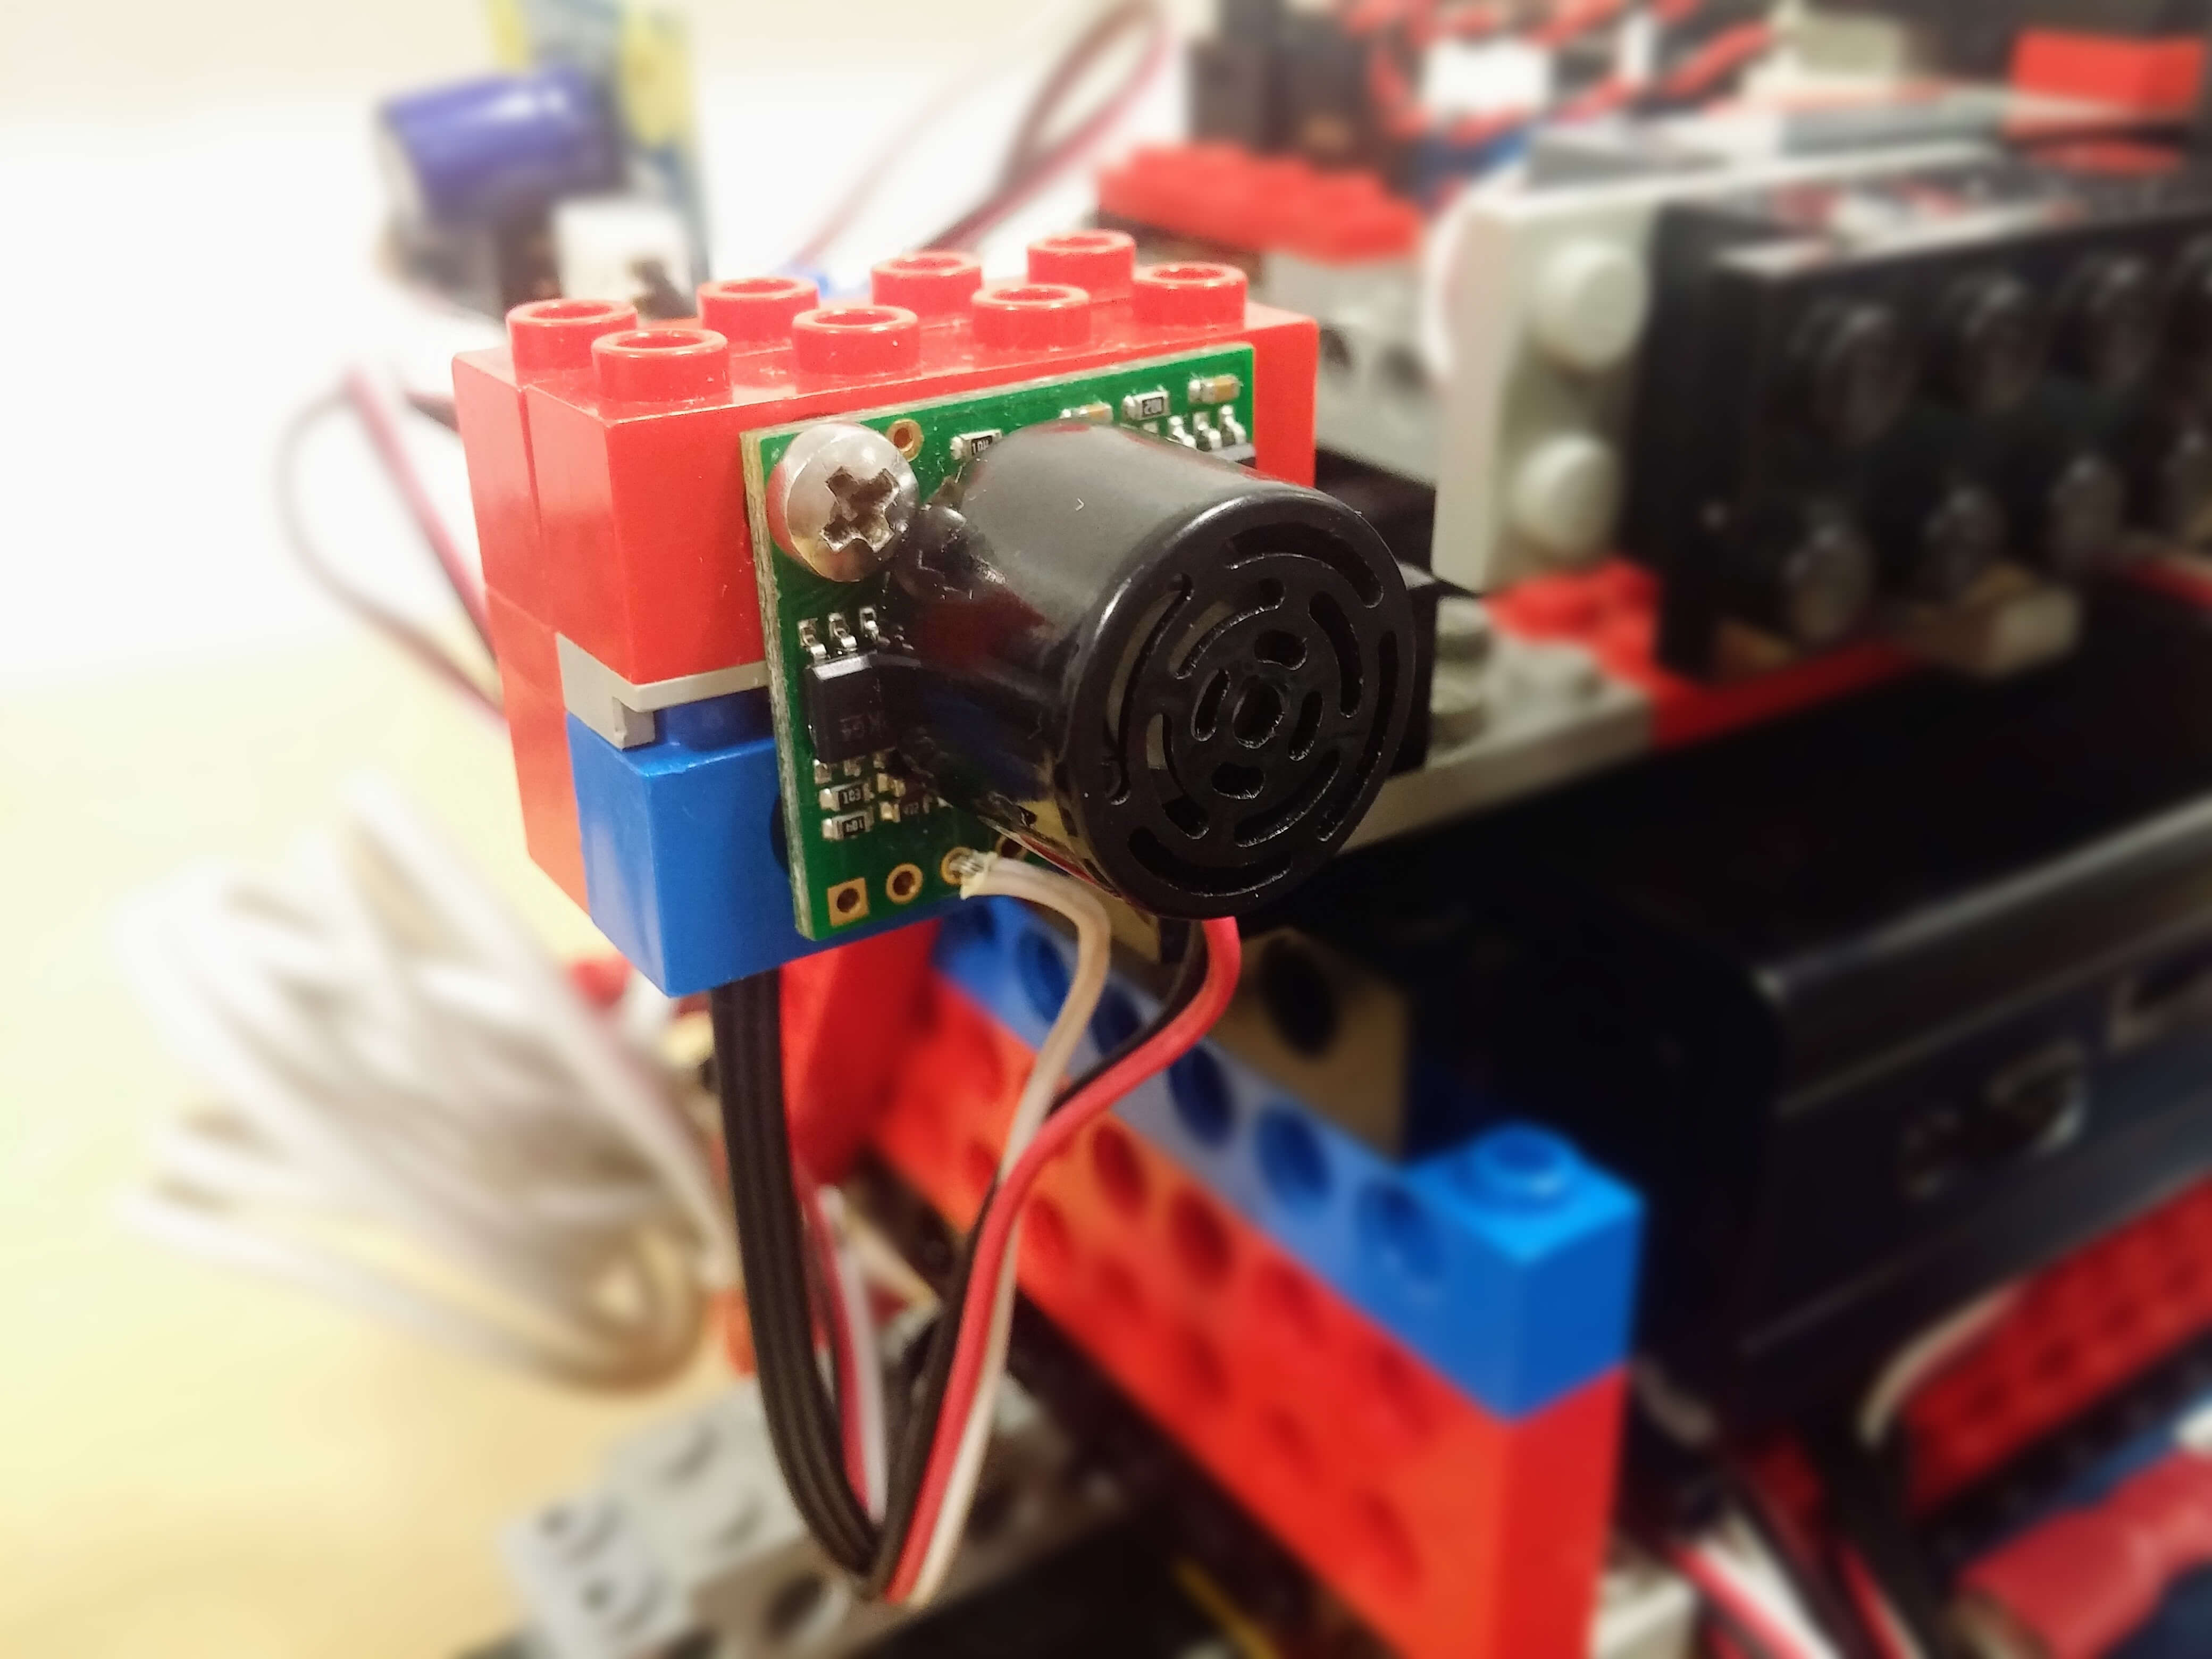
\includegraphics[width=0.7\linewidth]{res/robot-pics/sonar-placement.jpg}
    \caption{}
    \label{fig:}
\end{figure}

\subsubsection{Camera}

\begin{figure}[ht]
    \centering
    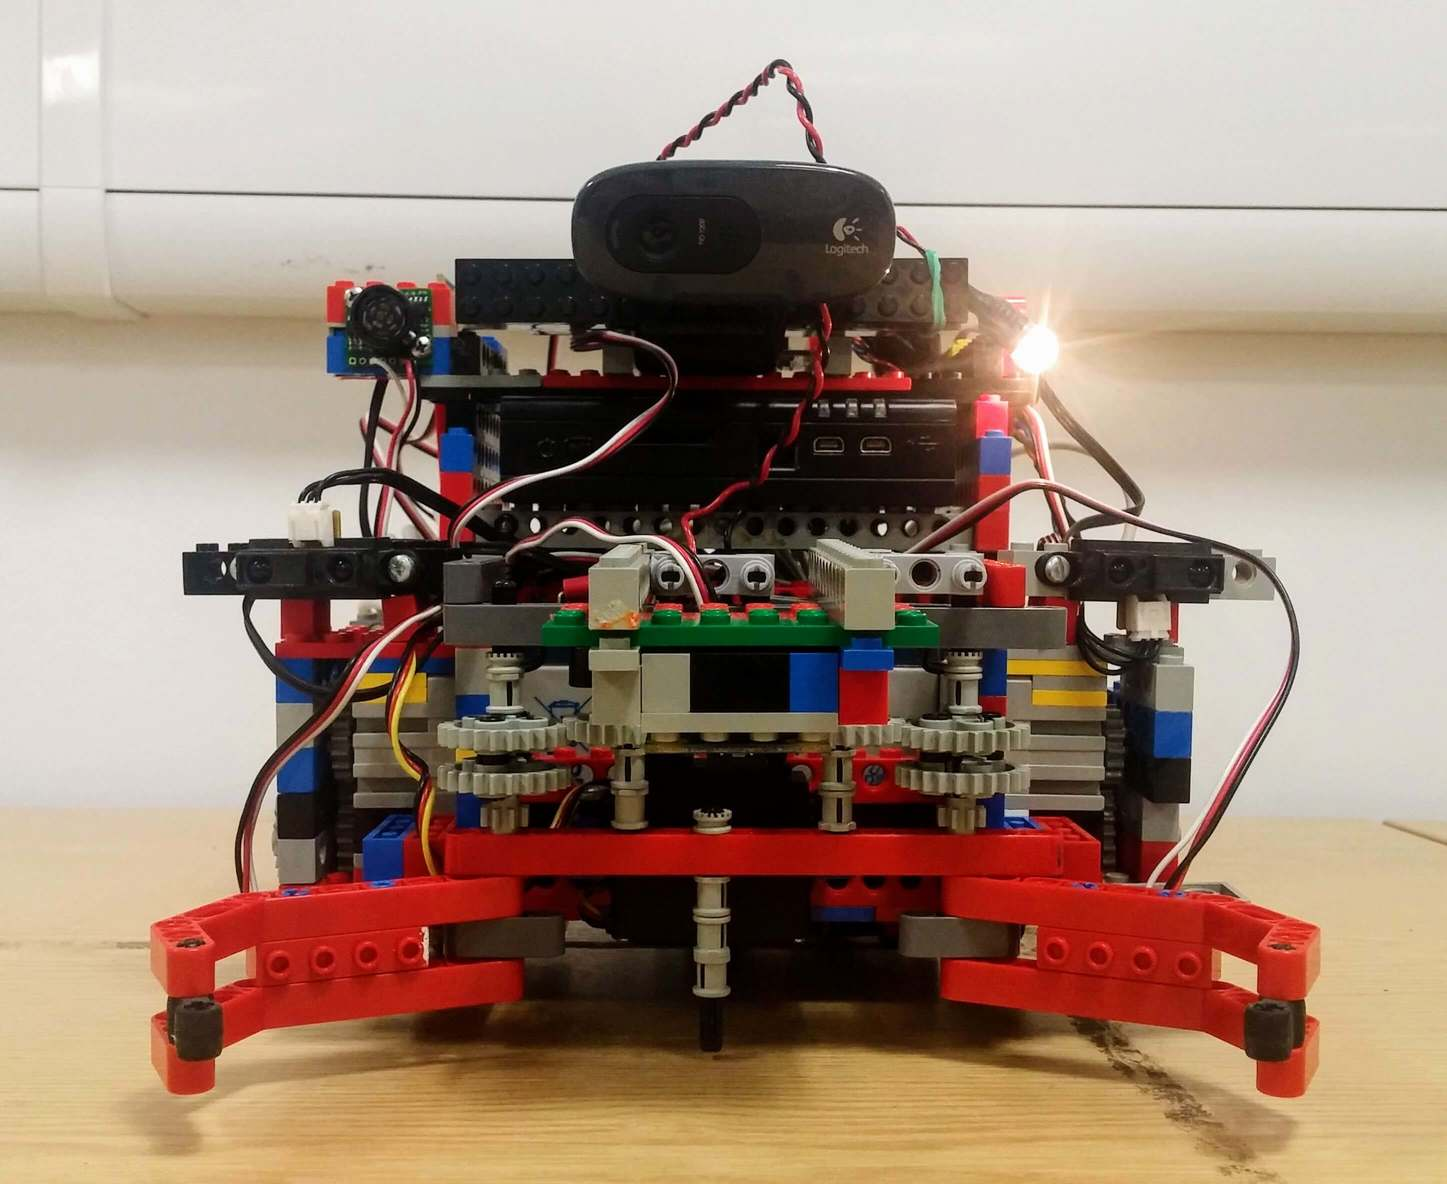
\includegraphics[width=0.7\linewidth]{res/robot-pics/view-front.jpg}
    \caption{}
    \label{fig:}
\end{figure}

\subsubsection{Hall effect sensor}

\begin{figure}[ht]
    \centering
    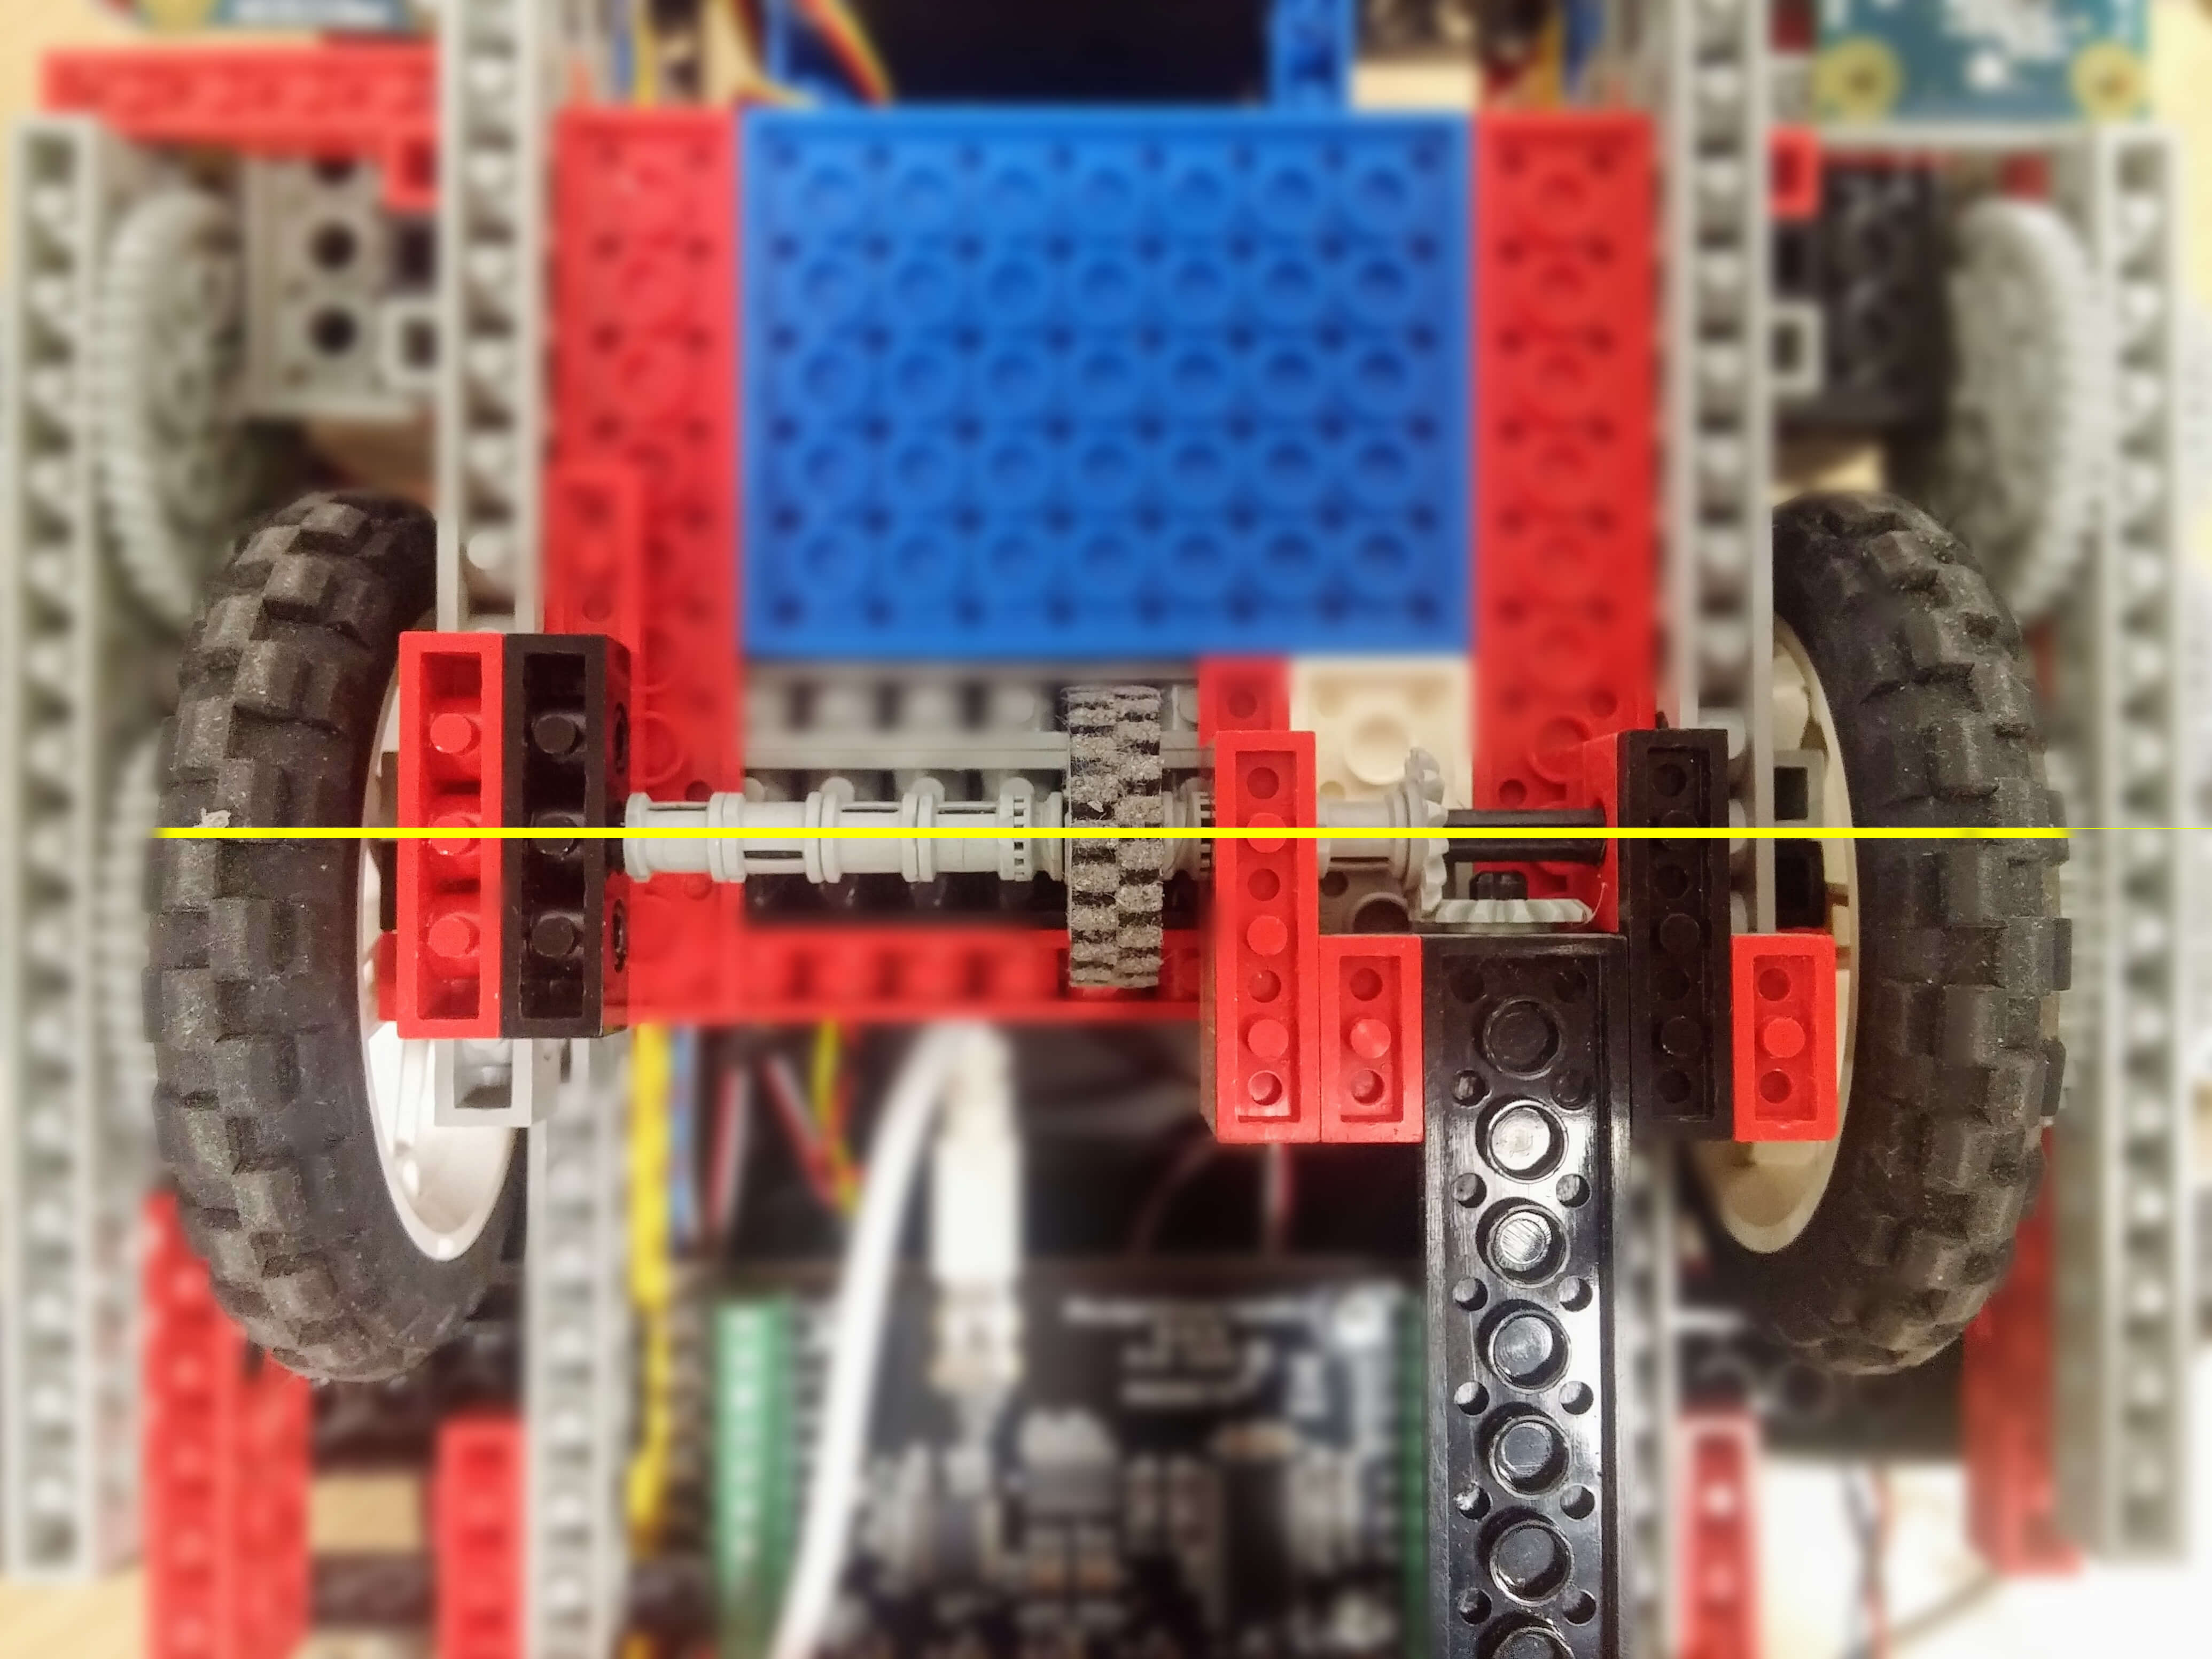
\includegraphics[width=0.7\linewidth]{res/robot-pics/pivot-wheel-layout.jpg}
    \caption{}
    \label{fig:}
\end{figure}

\begin{figure}[ht]
    \centering
    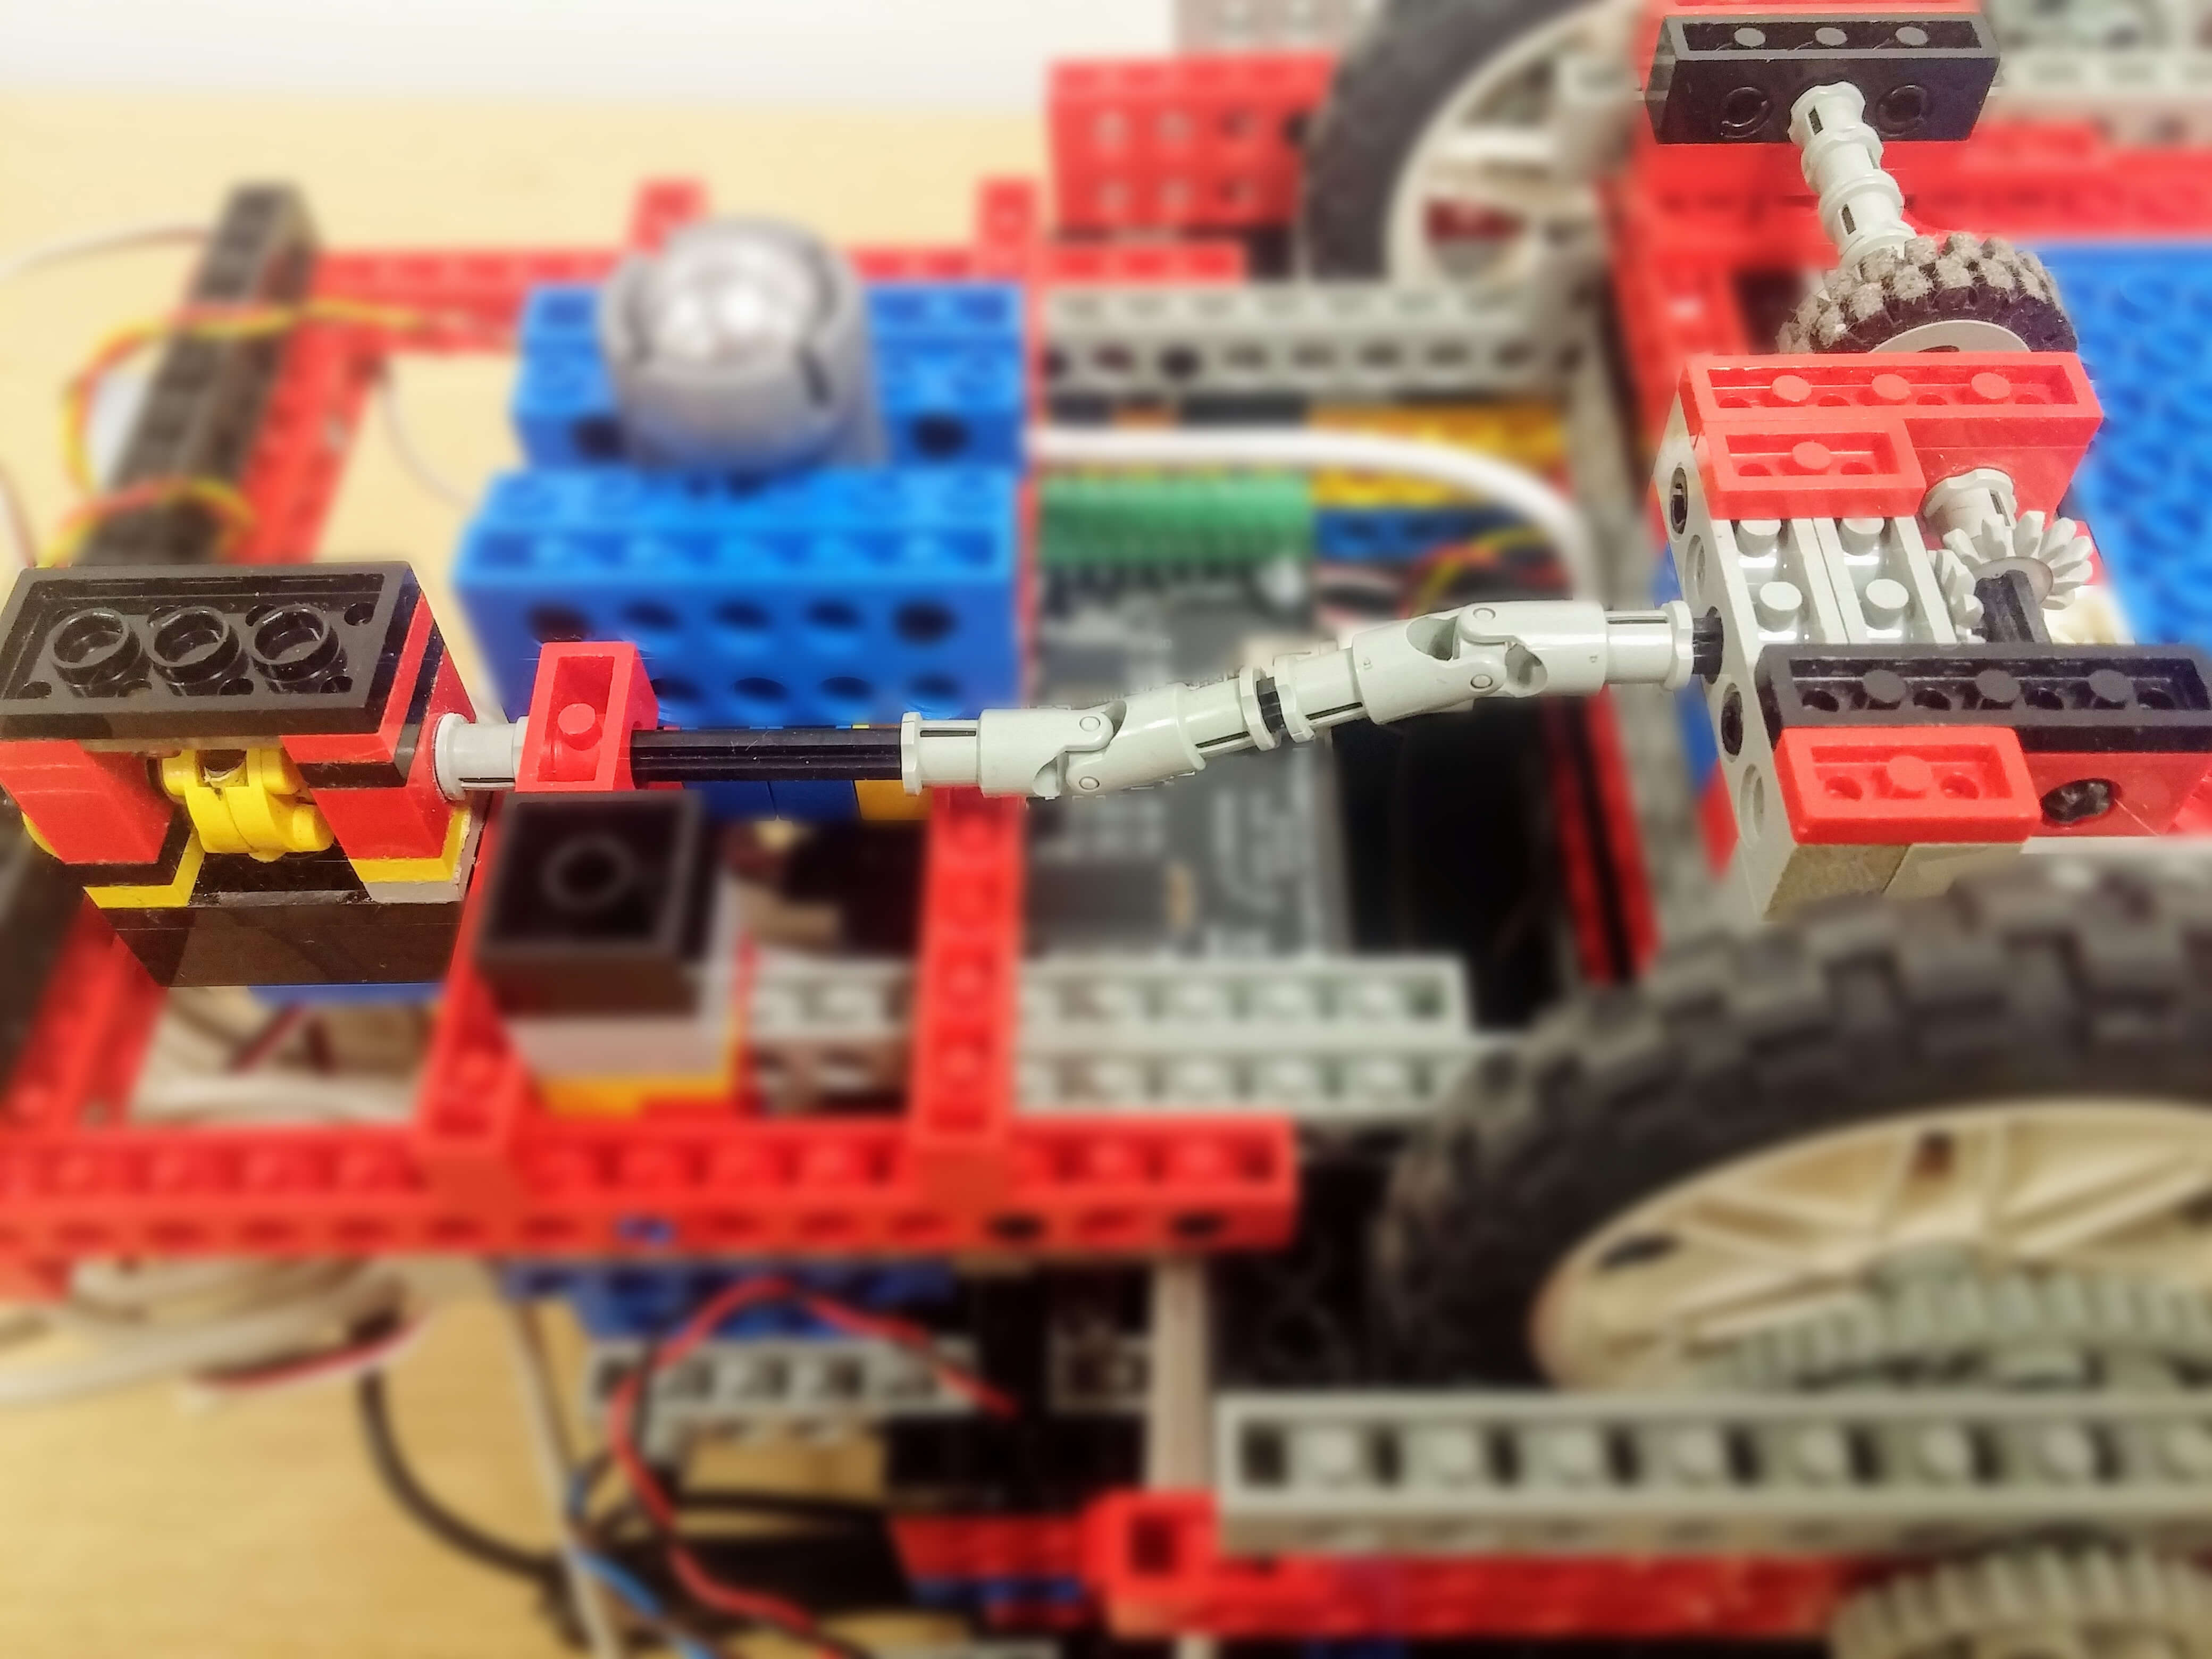
\includegraphics[width=0.7\linewidth]{res/robot-pics/pivot-wheel-sensor.jpg}
    \caption{}
    \label{fig:}
\end{figure}

\begin{figure}[ht]
    \centering
    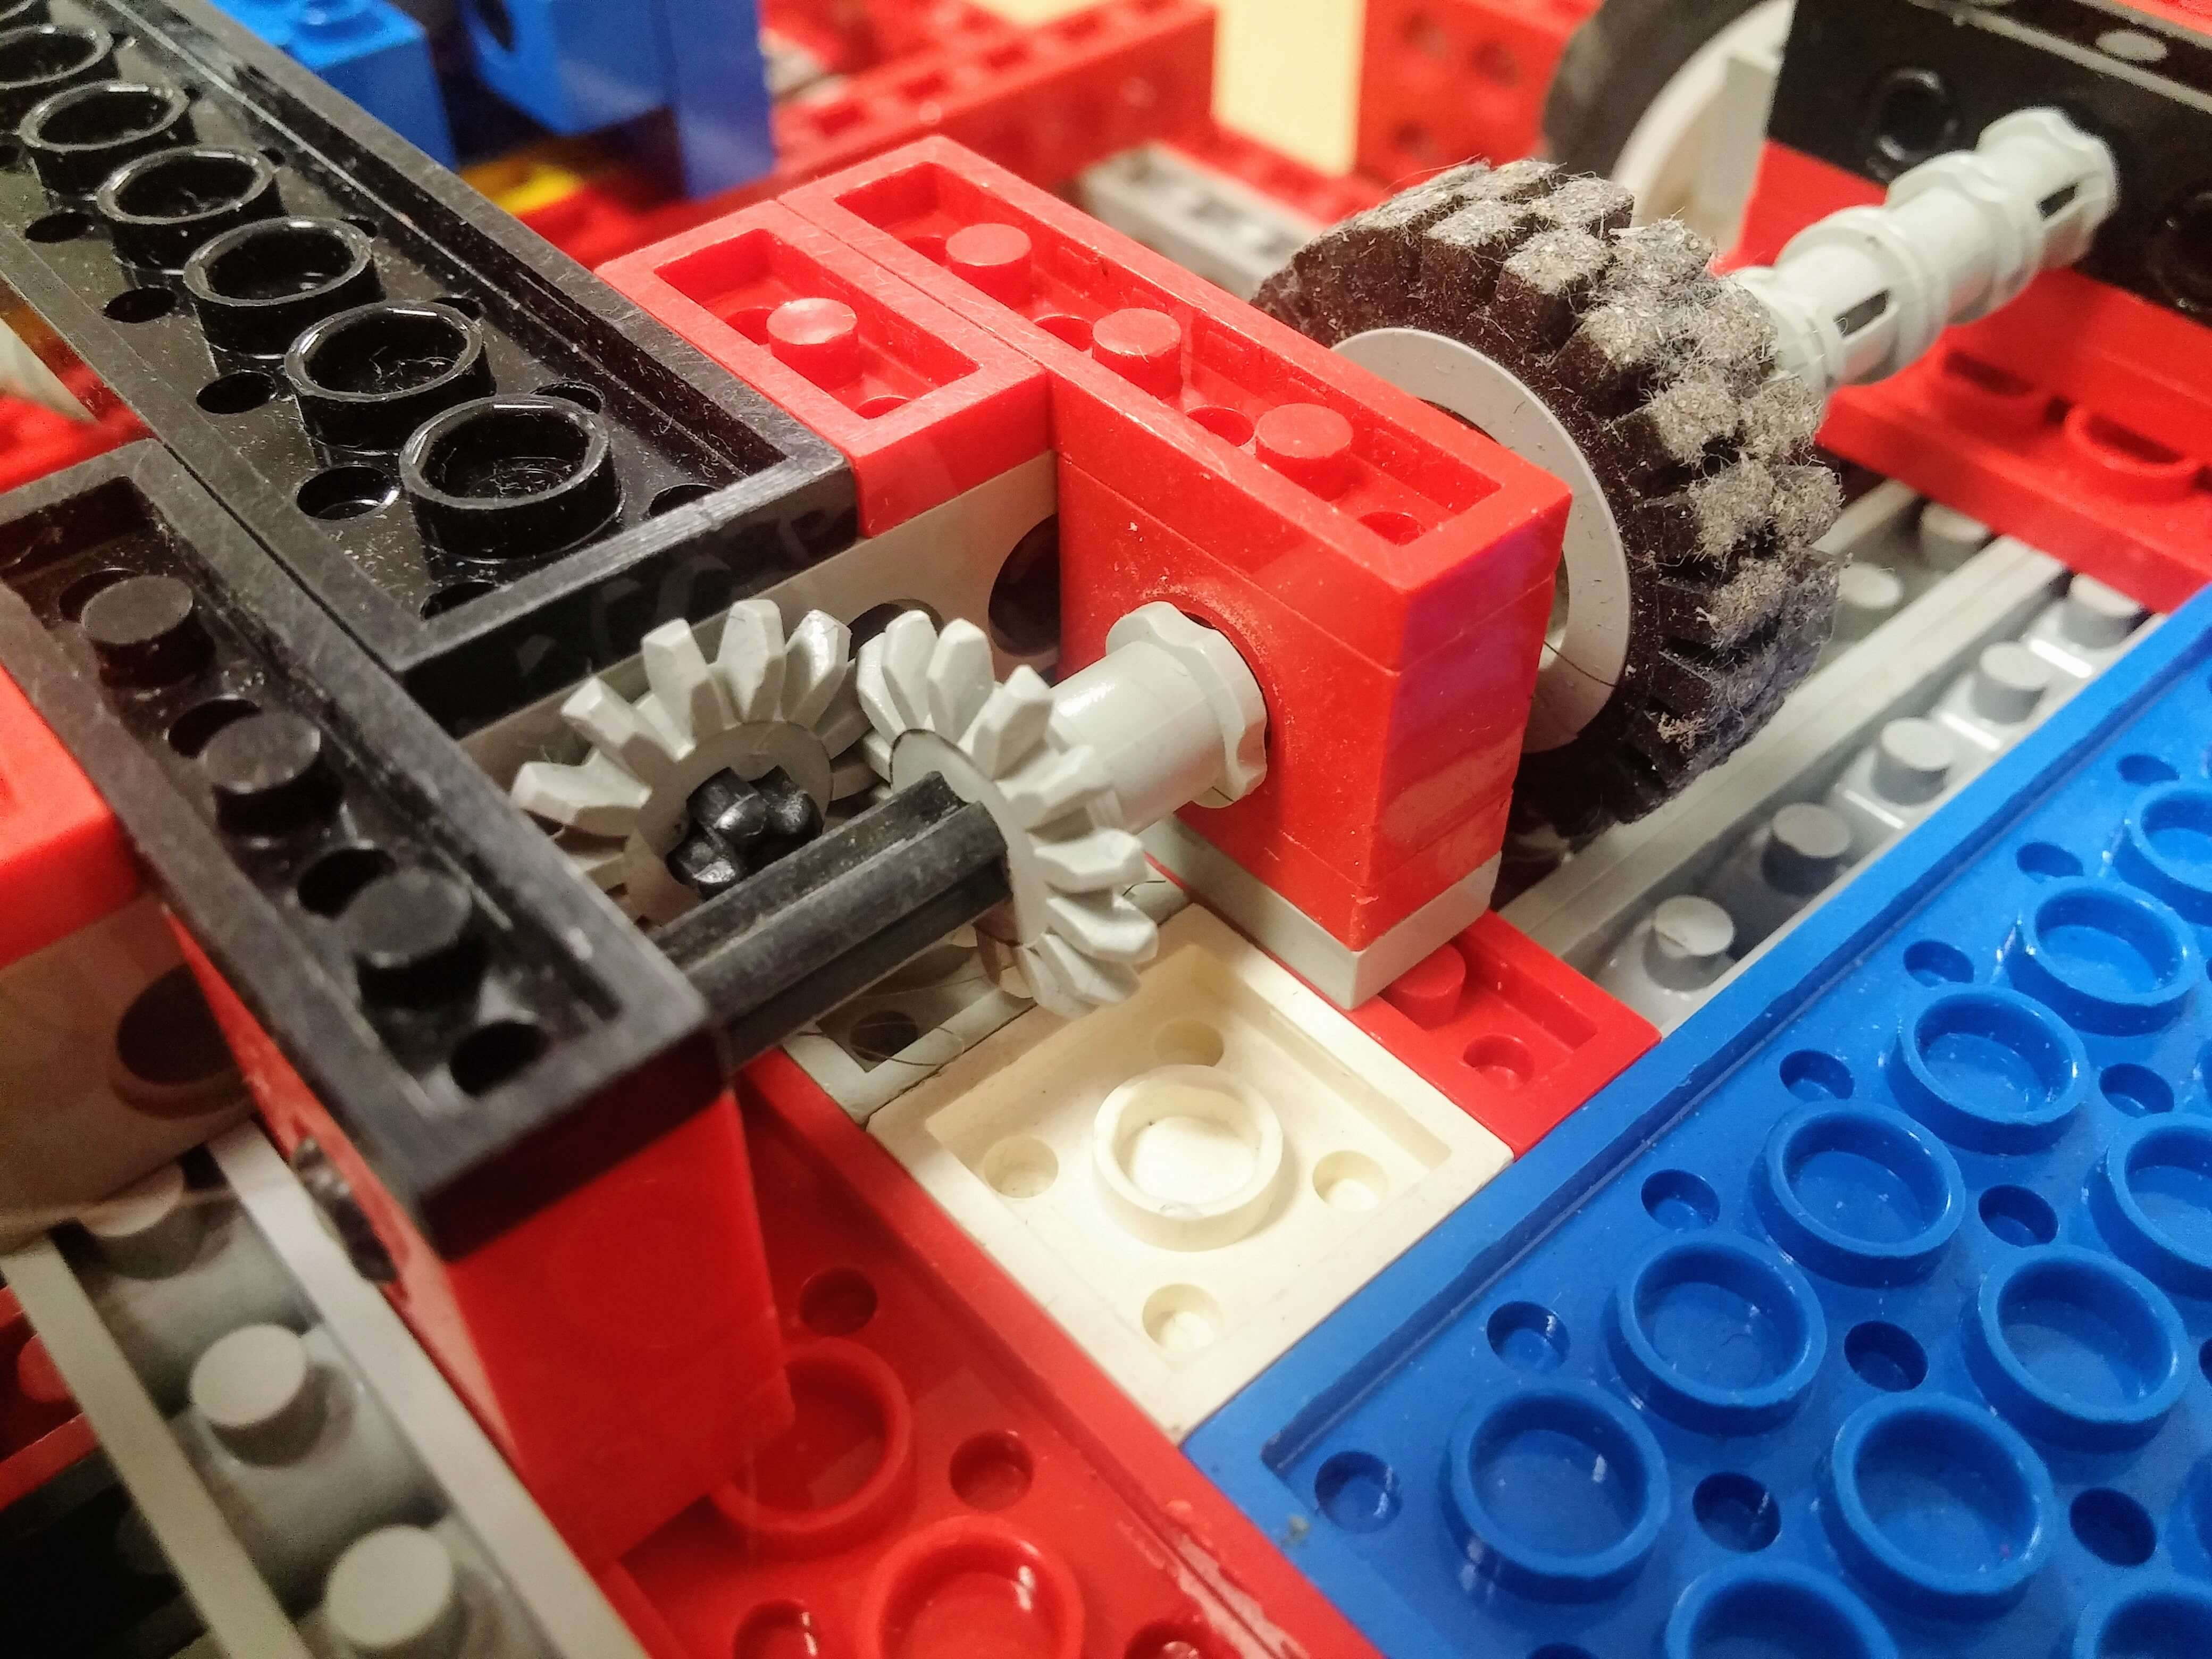
\includegraphics[width=0.7\linewidth]{res/robot-pics/pivot-wheel-axel-transfer.jpg}
    \caption{}
    \label{fig:}
\end{figure}

% - - - - - - - - - - - - - - - - - - - - - - - - - - -

For the control program you should provide a flow diagram or pseudo-code description, and again explain the reasoning that led to this solution.

This is likely to be the longest section of the report. Do not include code except for short snippets that help explain a crucial part of the program you created.

Avoid repetition and refer to other peoples' work instead of describing well known algorithms. (1400 words)

\newpage
